\section{Crypto Recap}
\subsection{Objectives:}
\begin{itemize}
  \item{\textbf{Confidentiality}}
  \item{\textbf{Integrity}}
  \item{\textbf{Authenticity}}
  \item{\textbf{Availability}}
  \item{Authorization}
  \item{Non-Repudiation, Accountability}
  \item{Freshness}
  \item{Anonymity, Unlinkability}
  \item{Intervenability, Contro}
  \item{Transparency}
\end{itemize}

\subsection{Confidentiality-Encryption}
\subsubsection{Symmetric Ciphers}
\begin{itemize}
  \item Secret key for en- and decryption
  \item Much more efficient
  \item \textbf{Block cipher: }encryps a plaintext block of fixed len e.g.: \textit{Advanced Encryption Standard (AES)}
  \item \textbf{Stream cipher: }encrypts a bitstream e.g.:\textit{ChaCha20}
\end{itemize}

\subsubsection{Asymmetric Ciphers}
\begin{itemize}
  \item Public key for encryption
  \item Private key for decryption
  \item Ex.: RSA-based encryption
\end{itemize}

\subsection{Integrity, Authenticity-Signatures, MACs}
\subsubsection{MACs}
\begin{itemize}
  \item Symmetric cryptography
  \item Protects data integrity \& authenticity
  \item Ex.: Hash-based MAC
\end{itemize}

\subsubsection{Digital Signatures}
\begin{itemize}
  \item Asymmetric cryptography
    \begin{itemize}
      \item{\textbf{Signing with} private key}
    \end{itemize}
  \item{Protects data integrity \& authenticity}
  \item{Provices non-repudation}
\end{itemize}

\subsection{Block Cipher Modes of Operation}
\subsubsection{Electronic Code Book (ECB)}
\begin{itemize}
  \item{Each plaintext block is encrypted seperatly}
  \item{Inherintly insecure! -> Smae block = Same cipher}
\end{itemize}

\subsubsection{Cipher Block Chainning (CBC)}
\begin{itemize}
  \item Plaintext is chained to previous ciphertext by XOR and encrypted afterwards
  \item Difficult to apply securely -> implementations often vulnerable
\end{itemize}

\subsubsection{Galois Counter Mode (GCM)}
\begin{center}
  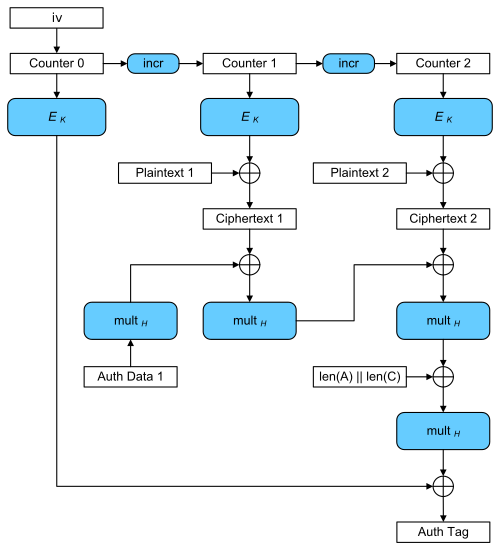
\includegraphics[width=0.5\columnwidth]{Resources/GCM-Galois_Counter_Mode_with_IV.svg.png}
\end{center}

\section{Tranport Layer Security (TLS)}
\subsection{TLS handshake protocol}
\begin{itemize}
  \item Parameter Negotiation
  \item Key exchange
  \item Authentication
\end{itemize}
\subsection{TLS record protocol}
\begin{itemize}
  \item Protection of integrity, authenticiy and confidentiality
  \item \textbf{Symmetric Cryptography:} e.g., block cipher, usually AES
\end{itemize}

\subsection{Attacks}
\begin{itemize}
  \item Attacks on the record layer
  \item Attacks on the session key
  \item Attacks on the private server key
    \begin{itemize}
      \item Attacks on implmentations: Timing Attacks, Heratbleed, Invalid Point Attacks
    \end{itemize}
  \item Attacks on TLs eco system
    \begin{itemize}
      \item Attacks on certificates and the PKI
      \item Attacks on the browser GUI
    \end{itemize}
\end{itemize}

\subsection{Overview TLS 1.0-1.2 \& TLS 1.3}
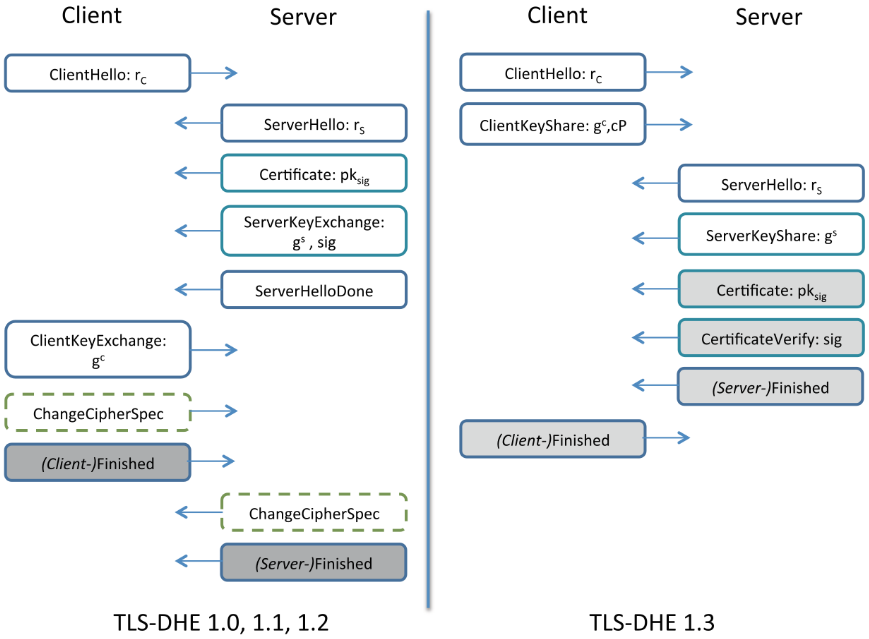
\includegraphics[width=0.8\columnwidth]{Resources/tls.png}

\subsection{HKDF Key Derivation Function}

\subsection{Forward Secrecy}
\begin{itemize}
  \item TLS 1.3 using certificate-based Authentification: \textbf{forward secrecy}
  \item TLS 1.3 using pre-shared keys (PSK):
    \begin{itemize}
      \item PSK using \textit{elliptic-curve} Diffie-Hellman: \textbf{forward secrecy}
      \item PSK without EC-DHE (symmetric-only) and zero-round-trip data: \textbf{no forward secrecy}
    \end{itemize}
\end{itemize}

\subsection{Datagramm TLS}
\begin{itemize}
  \item DTLS is identical to TLS where possible
  \item DTLS has to introcue new mechanisms
    \begin{itemize}
      \item Explicit sequence numbers
      \item Retransmission timer for handshake message
      \item Message re-ordering for the handshake
      \item Fragmentation of large handshake messages into serveral DTLS records
      \item Optional replay detection
      \item Invalid records are discarded (silently)
      \item Denial-of-Service countermeasures: statless cookies, HelloRetryRequest
    \end{itemize}
\end{itemize}

\section{Network Layer Security: IPsec}
\subsection{TLS limitations}
\begin{itemize}
  \item Does not protect all traffic between hosts
    \begin{itemize}
      \item Protects only a single connection; new connection => new key agreement or session resumption necessary
      \item Non-TCP traffic (resp. non-UDP trafic for DTLS) cannto be protected
    \end{itemize}
  \item Does not protect the TCP layer (RST attacks on TCP are possible which terminate TLS connection)
  \item Application specific: applications have to be modified to use TLS/DTLS
  \item Using a TLS-based tunel for VPNs has disadvangates (TCP) (DTLS good option tho)
\end{itemize}

\subsection{Overview IPsec}
\begin{itemize}
  \item Goal: Protect IP packets cryptographically
    \begin{itemize}
      \item Confidentiality
      \item Integrity \& Authenticity
    \end{itemize}
  \item Seperation of packet protection from key exchange
    \begin{itemize}
      \item Protocols for packet encryption and authentification:
        symmetric crypto, implemented in the TCP/IP stack
      \item Key Exchange completly unrelated:
        asymmetric (+symmetric) crypto, implemented as network daemon
    \end{itemize}
\end{itemize}
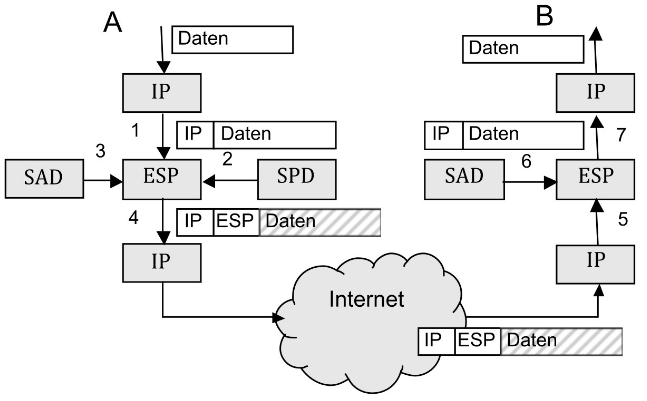
\includegraphics[width=\columnwidth]{Resources/ipsec_overview.png}

\subsection{Packet Formats and Operational Modes}
\subsubsection{Authentification Header (AH)}
\begin{itemize}
  \item Integrity \& Authenticity only
  \item Partially protects "outer" IP header
    \begin{itemize}
      \item Variable fields cannot be includes
        \begin{itemize}
          \item Flags, Fragment Offset, TTL, Header Checksume
        \end{itemize}
      \item Other fields are included in MAC computation
        \begin{itemize}
          \item Version, IP header length, total length, identification, Protocol (must be AH), source/dest Address
        \end{itemize}
    \end{itemize}
\end{itemize}
\subsubsection{Encapsulating Security Payload (ESP)}
\begin{itemize}
  \item Confidentiality, Integrity \& Authenticity
  \item Does not protect "outer" IP header
\end{itemize}
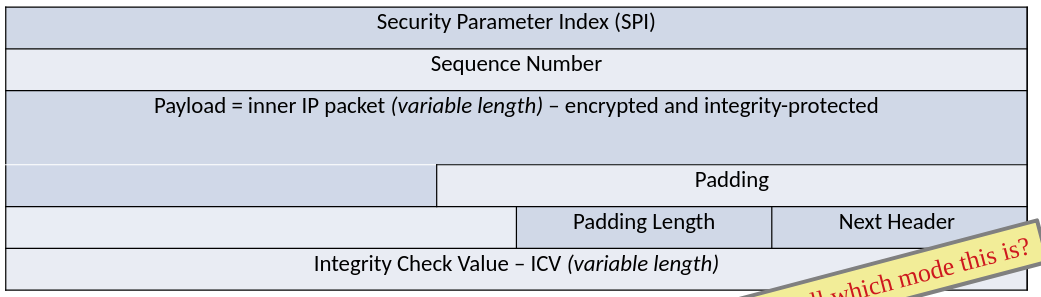
\includegraphics[width=\columnwidth]{Resources/esp.png}
\begin{itemize}
  \item SPI: SA-Identifier
  \item Next Header: type of payload data (e.g. IPV4)
  \item Integrity Check Value: data for authentification / integrity protection
    \begin{itemize}
      \item Message Authentification Code (MAC)
    \end{itemize}
  \item SAs are negotiated in the key exchange
  \item Sender side: Packet must be categorized to determine which SA applies (By parameters such as destination=)
  \item Receiver side: Determines SA from IPsec header of received packet
  \item SA Parameters:
    \begin{itemize}
      \item IPsec protocol (AH or ESP)
      \item Authentification alrogrithm and key
      \item Encryption algorithm and key
      \item IPsec mode (transport or tunnel)
      \item SA lifetimne
      \item Sequence number: current counter
      \item On reciver side: "Sliding Window" for replay protection
    \end{itemize}
\end{itemize}

\subsection{Scenarios}
\begin{itemize}
  \item Host to host
  \item Host to gateway
  \item Gateway to gateway
\end{itemize}

\subsection{The Internet Key Exchange (IKE)}
\begin{itemize}
  \item So far, keys are already exchanges, SAs negotiated... but how?
  \item Authentification of the communication endpoints
  \item Dynamic negotiation fo algorithms and parameters
  \item Key establishment
    \begin{itemize}
      \item Forward Secrecy
    \end{itemize}
  \item Resistance to DoW attacks
  \item Efficiency (computation, messages, round trips)
\end{itemize}

\subsection{IKEv1}
\begin{itemize}
  \item Phase 1: main mode vs. aggressive mode
  \item Authentification modes:
    \begin{itemize}
      \item Digital Signatures
      \item Public key encryption(PKE): two variants (rarely used)
      \item Pre-shared keys(PSK)
    \end{itemize}
  \item Phase 2 (quick mode)
    \begin{itemize}
      \item With DH (=> forward secrecy)
      \item Without DH (=> no forward secrecy)
    \end{itemize}
\end{itemize}
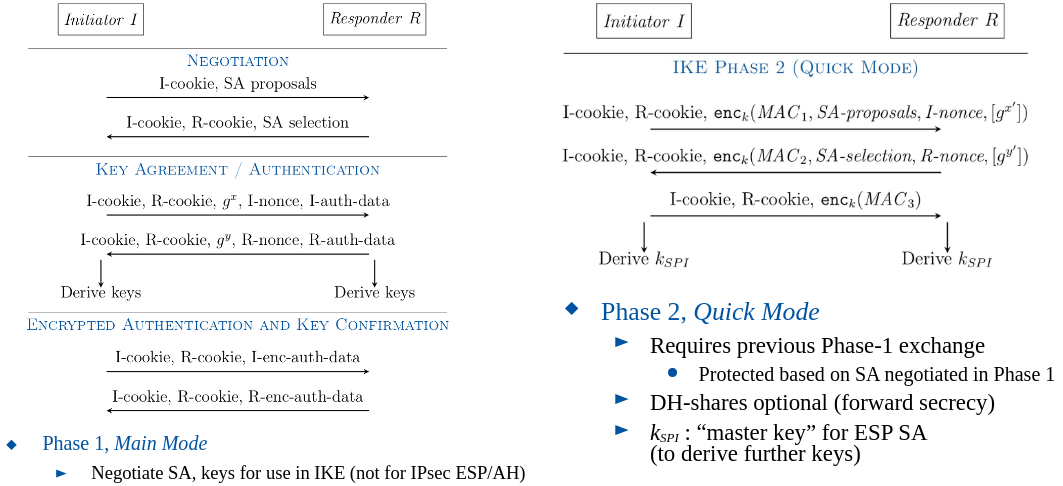
\includegraphics[width=\columnwidth]{Resources/ikev1.png}

\subsubsection{Discussion}
\begin{itemize}
  \item Complicated
    \begin{itemize}
      \item Information from serveral (complex) RFCs required
      \item Many options variants
    \end{itemize}
  \item Gneric
    \begin{itemize}
      \item Clean seperation of different phases and functionalities
        \begin{itemize}
          \item Can be advantagous in theory, but leads to inefficincies
        \end{itemize}
      \item Intended as general handshake and key agreement protocol, not only for IPsec
        \begin{itemize}
          \item In practice: only used for IPsec
        \end{itemize}
      \item Inneficient
        \begin{itemize}
          \item Requires too many round trips
        \end{itemize}
      \item Inadequate DoS protection
        \begin{itemize}
          \item IKEv1 uses stateful cookies
        \end{itemize}
    \end{itemize}
\end{itemize}

\subsection{IKEv2}
\begin{itemize}
  \item Phase 2 (partially) combindes with Phase 1
    \begin{itemize}
      \item More efficient thatn IKEv1
      \item Initial negotiation of IPsec SA included
    \end{itemize}
  \item Additional SAs can be negotiaded in furhter Phase 2 protocol runs
  \item Simplified specification
    \begin{itemize}
      \item Essential information in one RFC
      \item No distinction main mode vs. aggressive mode
    \end{itemize}
  \item DoS protection using statless cookies: optional
\end{itemize}
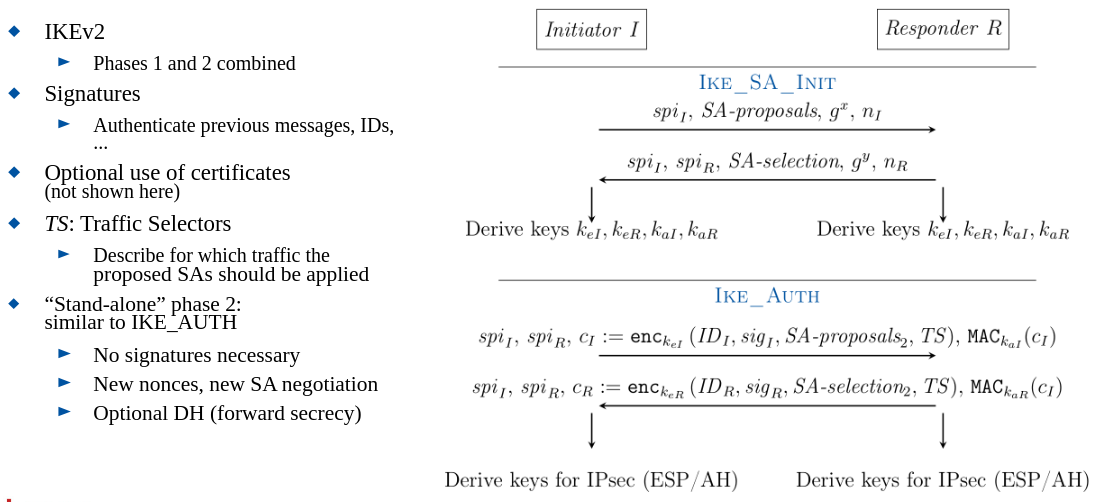
\includegraphics[width=\columnwidth]{Resources/ikev2.png}

\subsection{SA Proposals}
\begin{itemize}
  \item Serverl proposals possible
  \item Proposal contains transforms
  \item Differnten options for each transform possible
    \begin{itemize}
      \item Exactly one transform has to be selected
    \end{itemize}
\end{itemize}
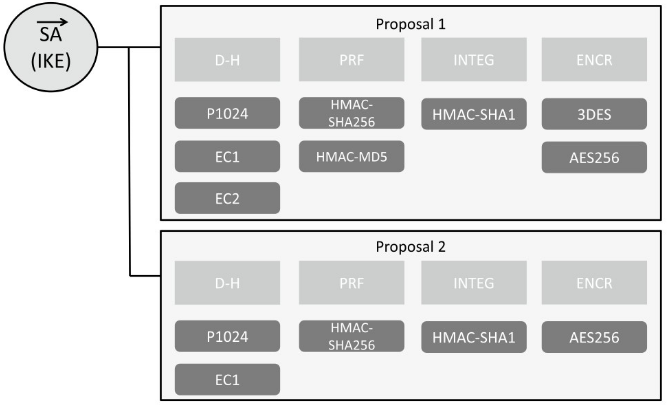
\includegraphics[width=0.7\columnwidth]{Resources/ike_sa_proposal.png}

\section{Security on Layer 2 (MAC Layer, Ethernet)}
\subsection{Attacks}
\begin{itemize}
  \item MAC address spoofing
  \item ARP spoofing
  \item ARP cache poisoning
\end{itemize}

\subsection{Network Access Control}
\begin{itemize}
  \item \textbf{Frontend} protocols: Cient -> Network Access Server
    \begin{itemize}
      \item Point-to-Point connections: PPP
      \item LAN: PPPoE, EAPoL
      \item WLAN: WPA/WPA2/WPA3, EAPoL
    \end{itemize}
  \item \textbf{Backend} protocols: Network Access Server --> Authentication Server AAA protocols (Authentication, Authorization, Accounting)
    \begin{itemize}
      \item Radius, Diameter
      \item TACACS+
    \end{itemize}
\end{itemize}
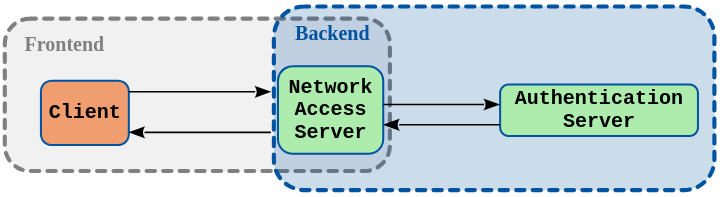
\includegraphics[width=0.6\columnwidth]{Resources/network_access_control.png}

\subsubsection{Radius - Remote Authentification Dial-In User Service}
\begin{itemize}
  \item Backend protocol
  \item Dial-In Server
    \begin{itemize}
      \item E.g. DSL
      \item Company infrastructure
    \end{itemize}
\end{itemize}
\textbf{Packet Format}\\
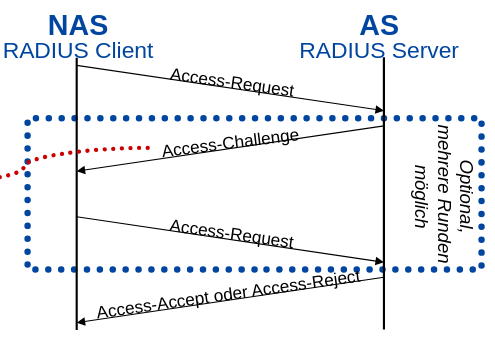
\includegraphics[width=0.7\columnwidth]{Resources/radius.png}
\textbf{Security}\\
\begin{itemize}
  \item Old protocol
    \begin{itemize}
      \item Tries to protect sesitive data only
      \item Insecure cryptography
    \end{itemize}
  \item Uses only over secure protocols
    \begin{itemize}
      \item Usually TLS
    \end{itemize}
  \item RADIUS successor: Diameter
    \begin{itemize}
      \item Fmore flexible, extensible, application-aware
      \item "Security" features removed, no more insecure crypto of RADIUS
        => To be used over secure protocols TLS/DTLS/IPsec
    \end{itemize}
\end{itemize}

\subsubsection{Point-to-Point Protocol (PPP)}
\begin{itemize}
  \item \textbf{PPP: }Frontend protocol to connect two devices
    \begin{itemize}
      \item Typically used for dial-up connections (e.g. DSL)
      \item Transported over Layer 2 protocol (e.g. ethernet)
    \end{itemize}
  \item Authentification mechanisms
    \begin{itemize}
      \item PAP: username/password
      \item CHAP: Challange Handshake Authentification Protocol
      \item EAP: Extensible Authentification Protocol
    \end{itemize}
  \item \textbf{PPPoE: }PPP over Ethernet (e.g. used for DSL connections)
    \begin{itemize}
      \item Discovery: Client negotiates session with network access server
      \item PPP Session: PPP frames are encapsulated in ethernet frames; potentially several hops
    \end{itemize}
\end{itemize}

\subsubsection{Extensible Authentification Protocol (EAP)}
\begin{itemize}
  \item Extensible authentification framework
    \begin{itemize}
      \item Fronted protocol for lcient authentification
      \item Server send request (e.g. challenge, ident. request, ..)
      \item Client responds
      \item Server sends success or failure message
      \item EAP messages can be transported in RADIUS messages (as RADIUS attribute) for backend communication
    \end{itemize}
  \item EAPoL: EAP over LAN
\end{itemize}

\subsubsection{Port Based Network Access Control (PNAC)}
\begin{itemize}
  \item Authentification of clients befre they can use the network (LAN)
    \begin{itemize}
      \item Client connect to the network
        \begin{itemize}
          \item Authentification traffic is allowed
        \end{itemize}
      \item Switch port can only be used for other purposes after successful authentification
      \item Re-authentification after timeouts, link-down, etc.
    \end{itemize}
  \item PNAC uses EAPoL
  \item Terminology: Port Access Entities (PAE)
    \begin{itemize}
      \item Client: supplicant
      \item Netowrk access server: authenticator
      \item Attention: "port"
    \end{itemize}
\end{itemize}

\subsection{MACsec}
\begin{itemize}
  \item cryptographically protect the ethernet layer
  \item Based on MACsec Key Agreeement (MKA)
    \begin{itemize}
      \item After successful authentification (typically EAP)
      \item Derives key from CAK - connectivity association key (pre-shared)
      \item Key can be set up by EAP (e.g. EAP-TLS)
    \end{itemize}
\end{itemize}
 \subsubsection{Frame}
 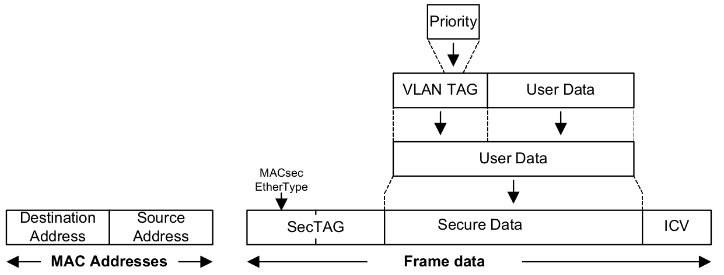
\includegraphics[width=0.8\columnwidth]{Resources/macsec_frame.png}
 \begin{itemize}
  \item Data cen be encryped and/or authentificated
  \item AES-GCM is supported
 \end{itemize}
 \textbf{Security TAG (SecTAG)}\\
 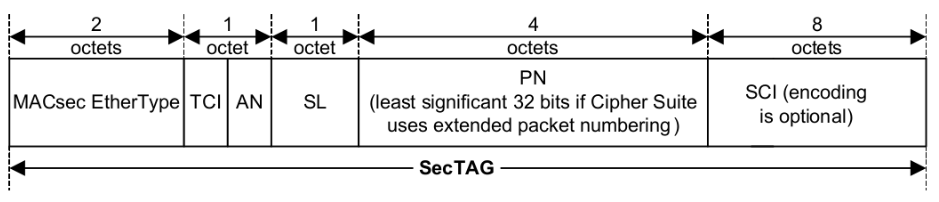
\includegraphics[width=0.8\columnwidth]{Resources/sec_tag.png}
 \begin{itemize}
  \item TCI: TAG Control Information
  \item AN: Association Number
  \item SL: Short Length (payload length; for short frames only)
  \item PN: Packet Number
  \item SCI: Secre Channel Identifier (edentify SA, when CA needs ore than 4)
    \begin{itemize}
      \item SA is identified by SCI (optional) and AN
    \end{itemize}
 \end{itemize}
 \subsection{Summary}
\begin{itemize}
  \item Security on Layer 2 can protect all higher Layer
    \begin{itemize}
      \item But: only in same network
      \item Does nt work accross Layer 3 routers
    \end{itemize}
  \item Network Access Control protects access to the network
    \begin{itemize}
      \item Client Authentification
      \item RADIUS/DIAMETER
      \item EAP
      \item Port-Based Access Control
    \end{itemize}
  \item MACsec protects traffic
  \begin{itemize}
    \item Encryption \& authentification
  \end{itemize}
\end{itemize}

\section{Wireless Security}
\subsection{WiFi Security}
\subsubsection{Historic Overview}
\begin{itemize}
  \item 1999: WEP (Wired Equivilaent Privacy)
    \begin{itemize}
      \item Goal: "as secure as a wired LAN"
      \item Insecure, various attacks known
    \end{itemize}
  \item 2003: WPA (WiFi Protected Access)
    \begin{itemize}
      \item Improved protocols; most known attacks on WEP prevented
      \item Enterprice Mode
      \item But: Requirement ofr hardware-compatibility with WEP devices => Encryption improved, but still based on obsolete stream cipher
    \end{itemize}
  \item 2004: WPA2 (still used) 
    \begin{itemize}
      \item Similar to WPA, but AES-based encryption: AES-CCMP
    \end{itemize}
  \item 2018: WPA3 (supported by new devices) 
    \begin{itemize}
      \item Serveral improvements: 
        Prevention of offline-attacks on pre-shared keys, forward secrecy, encryption for "open" WLANs
    \end{itemize}
\end{itemize}
\subsubsection{WPA/WPA2 Security}
\begin{itemize}
  \item Personal Mode
    \begin{itemize}
      \item Pre-Shared Keys
    \end{itemize}
  \item Enterprise Mode 
    \begin{itemize}
      \item EAP-TLS, PEAP, EAP-TTLS
    \end{itemize}

\textbf{AES-CCMP}\\
  \item Authenticated Encryption with Associated Data (AED)
  \item AES-CCM
    \begin{itemize}
      \item Authentication: CBC-MAC
      \item Encryption: Counter Mode (CTR)
      \item MAC and encyprion: computed simultaneously
    \end{itemize}
\end{itemize}

\textbf{4-Way Handshake}\\
\begin{itemize}
  \item Based on Pairwise Master Key (PMK)
    \begin{itemize}
      \item Personal Mode (WPA-PSK):
        Computed from passphrase and SSID (as "salt") using PBKDF2 (password-based key derivation function)
      \item Enterprise Mode: Established by key exchange protocol (e.g. EAP-TLS, PEAP)
    \end{itemize}
  \item 4-Way HS to derive Pairwise Transient Key (PTK) 
    \begin{itemize}
      \item Exchance nonces
      \item PTK is derived by hashing PMK, nonces, MAC addrs 
      \item Furhter key (for differnet purposes) derived from PTK 
      \item Client gets Group Temporary Key from AP (encrypted) 
      \item Message Integrity Code(MIC): MACs for integrity protection, key confirmation 
    \end{itemize}
  \item KRACK (2018): Key reinstallation attacks => meanwhile prevented by software/firmware updates 
  \item Problem: Offline attacks against passphrase 
\end{itemize}

\subsubsection{WPA 3 Improvements}
\begin{itemize}
  \item Mandatory Protected Managment Frames
    \begin{itemize}
      \item Prevents deauthentication attacks (DoS)
    \end{itemize}
  \item Replace PSK Authentication with SAW protocol 
    \begin{itemize}
      \item Simultaneous Authentication among Equals (SAE):
        "Dragonfly" handshake
      \item Prevents offline attacks on passphrase 
      \item Based on elliptic curve cryptography by default
    \end{itemize}
  \item Forward Secrecy based on Diffie-Hellman 
  \item 192-bit Security Mode (optional) 
    \begin{itemize}
      \item AES-256 (GCM)
      \item SHA-384 
      \item 284-bit elliptic curves or RSA with at least 3K bits 
    \end{itemize}
\end{itemize}

\subsubsection{Simultaneous Authentication among Equals}
\begin{itemize}
  \item SAE "Dragonfly" authenicates participants and establishes PMK
    \begin{itemize}
      \item Based on passphrase and (EC-)Diffie-Hellman
      \item Can be initiated simultaneously by both parties (useful for mesh networking) 
    \end{itemize}
  \item 4-Way Handshake 
    \begin{itemize}
      \item Esablishes PTK basen on PMK
      \item Same as in WPA2 
      \item But now: PMK with much higher entropy => Offlione attacks not practical 
    \end{itemize}
  \item Hash-to-Group: "Hunting and Pecking" 
    \begin{itemize}
      \item Generate point on elliptic curve from pasphrase (and MAC addresses, etc.)
      \item Cryptographic has function generates pseudo random numbers (by including a counter in the input) 
        \begin{itemize}
          \item Both parties must use the exact same inputs in the same order
        \end{itemize}
      \item Fixed procedure to derive x-coordinate 
        \begin{itemize}
          \item Check if point on curve can be generated
          \item If check fails: increase coutner and try again 
        \end{itemize}
    \end{itemize}
  \item Auth-Commit messages
    \begin{itemize}
      \item Exchange ECDH shares
    \end{itemize}
  \item Auth-Confirm messages 
    \begin{itemize}
      \item Key confirmation, authentication of messages
    \end{itemize}
\end{itemize}

\subsection{Bluetooth Security}
\begin{itemize}
  \item Authentication: device authentication, no user authentication
  \item Pairing/bondig: create shared keys; used in connections later on 
  \item Confidentiality: encryption of BT communication 
  \item Message Integrity: MACs (authenticated encryption) to protect BT communication 
  \item Authorization: control access to resources (based on devices, not users) 
  \item Security Modes 
    \begin{itemize}
      \item Mode 1: no security
      \item Mode 2: service level (only for backward compatibility) 
      \item Mode 3: link-level enforces security (only for backward compatibility) 
      \item Mode 4: authenticated link key using "Secure Connections", based on device pairing 
    \end{itemize}
  \item Eavesdropptin not trivial: Bluetooth uses frequency hoppting (not a security feature) 
\end{itemize}

\subsubsection{Device Pairing}
\begin{itemize}
  \item Authentication and generation of link key / long term key
  \item PIN/Legacy Pairing: enter PIN on both devices 
    \begin{itemize}
      \item Key generation based on PIN, device address, and random values
    \end{itemize}
  \item Secure Simple Pairing (SSP): since Bluetooth 2.1 
    \begin{itemize}
      \item Numeric Comparison
        \begin{itemize}
          \item Compare 6-digit numbers
        \end{itemize}
      \item Passkey Entry 
        \begin{itemize}
          \item Read 6-digit form one device, enter on the other one
        \end{itemize}
      \item Just Works 
        \begin{itemize}
          \item User accepts connection without verification
        \end{itemize}
      \item Out of Band (OOB) 
        \begin{itemize}
          \item Transmit data using other communication channels (e.g. NFC)
        \end{itemize}
    \end{itemize}
\end{itemize}

\subsubsection{Simple Secure Pairing (SSP)}
\begin{itemize}
  \item Unauthenticated ECDH
  \item 2-Stage Authentication 
    \begin{itemize}
      \item Stage 2: depends on pariing method
      \item Stage 2: Cryptographic authentication based on Stage 1 values and ECDH secret 
    \end{itemize}
  \item Key derivation to generate link key / long term key 
\end{itemize}

\subsubsection{Secure Authentication}
\begin{itemize}
  \item Paired (bonded) devices authenticate each other
  \item Challange-Response scheme 
    \begin{itemize}
      \item 128-bit random challanges
      \item Response: HMAC of BT addresses and challanges (using link key from pairing) 
        \begin{itemize}
          \item Before Bluetooth 4.1: based on Bluetooth-specific algorithm E1
        \end{itemize}
    \end{itemize}
  \item Authenication failure: introcude delay (exponential back-off) 
\end{itemize}

\subsubsection{Confidentiality}
\begin{itemize}
  \item Bluetooth-specific stream cipher E0
    \begin{itemize}
      \item Designed for efficiency
      \item Serious attacks hve been published 
      \item "Practical" in theory (but complex, hard to apply in practice) 
    \end{itemize}
  \item AES-CCM 
    \begin{itemize}
      \item Used since Bluetooth 4.1
      \item Key derived from link key (pairing) and the authentication step 
    \end{itemize}
\end{itemize}

\subsubsection{Privacy}
\begin{itemize}
  \item Privacy problem: Devices (users) can be identified by Bluetooth MAC addresses
  \item Mitigation: BLE private device addresses 
    \begin{itemize}
      \item Resolvable Private Address (RPA) is changed periodically
      \item Identity Address remains constant (but is not transmitted over the air) 
      \item Identity Resolving Key to map RPA to Identity Address 
      \item Especially imprtant to discoverable devices (which advertice identity info) 
    \end{itemize}
\end{itemize}

\subsubsection{5.x Security}
\begin{itemize}
  \item No major changes to security protocols and algorithms
  \item Bluetooth 5.0 
    \begin{itemize}
      \item PHY improvements, no relevant security changes
    \end{itemize}
  \item Bluetooth 5.1 
    \begin{itemize}
      \item HCI support for debug keys (should not be relevant in production systems)
    \end{itemize}
  \item Bluetooth 5.2: adds new features (Extended Attributes, Isochronous Communication, ...)
    \begin{itemize}
      \item Isochronous communication: connection-oriented or connection-less
        \begin{itemize}
          \item Group communication: group keys need to be established
          \item Broadcast Authenication 
        \end{itemize}
    \end{itemize}
  \item Bluetooth 5.3: Key Size Negotiation 
    \begin{itemize}
      \item Enables host to define minimun key size
    \end{itemize}
\end{itemize}
\subsubsection{BLUFFS}
\begin{itemize}
  \item BLUFFS: New attacks against bluetooth
    \begin{itemize}
      \item Breaks Forward Secrecy and Future Secrecy
      \item Enables man-in-the-middle attacks, impersonation if one session key compromised 
      \item Forces weak key: spec allows minimus of 7 Bytes entropy (56 Bits) 
        \begin{itemize}
          \item Brute-force attack: offline, parallelizable
          \item Forces reuse of compromised key 
        \end{itemize}
      \item Attack against bluetooth spec (BR/EDR: "Bluetooth Classic" versions 4.2 to 5.4): All compliant devices are affected 
      \item Published and presented at ACM CCS 2023 
    \end{itemize}
\end{itemize}

\subsubsection{implementations Vulnerabilities}
\begin{itemize}
  \item BlueBorn(2017): Collection of implementation Vulnerabilities
    \begin{itemize}
      \item On Windows, IOS, Linux, Android
      \item Buffer overflow, integer overflows, .. 
    \end{itemize}
  \item Android (2018): implementation flaws in L2CAP and SMP 
    \begin{itemize}
      \item Remote Memory Disclousure
    \end{itemize}
  \item BleedingTooth(2020): several bugin in Linux 
    \begin{itemize}
      \item Can even lead to arbitrary code execution in kernal mode
    \end{itemize}
  \item Windows (2021): BT Driver Elevation of Privilege 
  \item BrakTooth(2021) 
    \begin{itemize}
      \item Bluetooth controllers: SoC firmware Vulnerabilities(Link Manager)
      \item Estimation 1400 bluetooth chips/modules affected 
    \end{itemize}
\end{itemize}

\subsubsection{Summary}
\begin{itemize}
  \item Complex protocol stack, not easy to implement
  \item Many attacks in the past  
    \begin{itemize}
      \item on cryptography algorithms
    \end{itemize}
  \item Bluetooth versions before 2.1 are basically completely insecure 
  \item Bluetooth versions sinde 4.2 are relativly secure (...but: "BLUFFS"!) 
    \begin{itemize}
      \item But the implementations not necessarily!
    \end{itemize}
  \item Bluetooth 5.2 architecture similar to 4.x 
    \begin{itemize}
      \item Introduces new features and minor security improvements
    \end{itemize}
\end{itemize}

\section{Security Mobile Networks}
\subsection{Overview}
\begin{itemize}
    \item[\(\diamond\)] \textbf{First generation:} \emph{analog telephony networks} (voice only)
    \item[\(\diamond\)] \textbf{2\textsuperscript{nd} generation (2G):} \textcolor{blue}{GSM} \textit{~1990s}
    \begin{itemize}
        \item[\(\blacktriangleright\)] Digital, circuit-switched, SIM-based; introduced \textbf{cryptographic protection}
        \item[\(\blacktriangleright\)] “Generation 2.5”: \textcolor{blue}{GPRS} (packet-switched data traffic)
        \item[\(\blacktriangleright\)] “Generation 2.75”: \textcolor{blue}{EDGE} (increased bandwidth)
    \end{itemize}
    \item[\(\diamond\)] \textbf{3\textsuperscript{rd} generation (3G):} \textcolor{blue}{UMTS} \textit{~2000s}
    \begin{itemize}
        \item[\(\blacktriangleright\)] Much higher bandwidth
        \item[\(\blacktriangleright\)] Improved security: \textbf{mutual authentication}, better crypto algorithms
        \item[\(\blacktriangleright\)] “Generation 3.5”: \textcolor{blue}{HSDPA/HSUPA} (increased bandwidth)
    \end{itemize}
    \item[\(\diamond\)] \textbf{4\textsuperscript{th} generation (4G):} \textcolor{blue}{LTE} \textit{~2010s}
    \begin{itemize}
        \item[\(\blacktriangleright\)] Higher bandwidth
        \item[\(\blacktriangleright\)] Completely new \textbf{IP-based} core network
        \item[\(\blacktriangleright\)] Changes to security
    \end{itemize}
    \item[\(\diamond\)] \textbf{5\textsuperscript{th} generation (5G):} \textit{~2020-?}
    \begin{itemize}
        \item[\(\blacktriangleright\)] ... even better, of course ;-) ...
    \end{itemize}
\end{itemize}

\subsection{GSM Network}
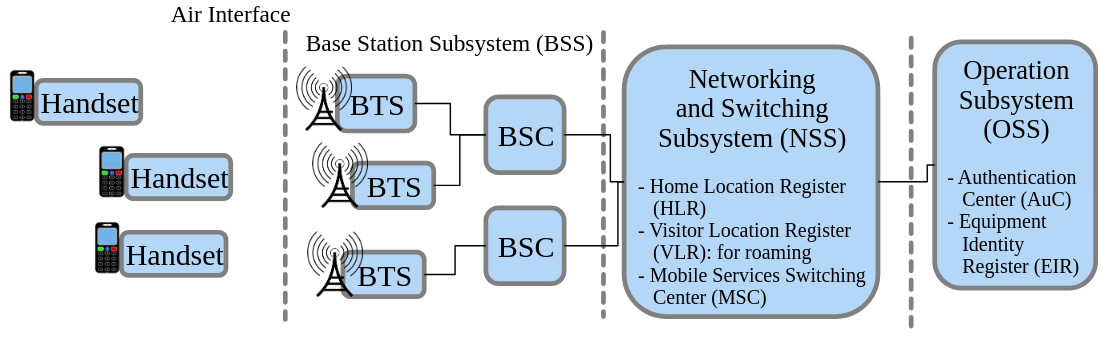
\includegraphics[width=0.9\columnwidth]{Resources/gsm.png}\\
BTS: Base Tranceiver Station\\
BSC: Base Station Controller\\
\begin{itemize}
  \item Circuit-switched network, designed for voice communication
    \begin{itemize}
      \item Stable channel between communication partners is reserved
      \item Seperate channel for signaling (different time slices)
      \item Slow, expensive
      \item GSM introduces SMS: small texts can be transferred in signaling channel
    \end{itemize}
\end{itemize}

\subsubsection{Secuirty}
\begin{itemize}
  \item Goal: "At least as secure as a landline"
  \item Security functions
    \begin{itemize}
      \item Autentication and Key Agreement (AKA)
        \begin{itemize}
          \item Shared secren in AuC and SIM
          \item Authentication via challange-response protocol
          \item "Agreement" on short term session keys for encryption
        \end{itemize}
      \item Confidentiality Protection
        \begin{itemize}
          \item Encryption of user data ("user plane")
          \item Encryption of signalling ("control plane")
        \end{itemize}
      \item Integrity Protection
        \begin{itemize}
          \item Only for signalling
          \item Often "implicitly" by encryption
        \end{itemize}
    \end{itemize}
\end{itemize}

\subsubsection{(U)SIM}
\begin{itemize}
    \item \textbf{SIM card} introduced with \textbf{GSM}
    \begin{itemize}
        \item \textbf{SIM:} \emph{Subscriber Identity Module}
        \item \textbf{International mobile subscriber identity (IMSI)}
        \begin{itemize}
            \item \emph{Temporary mobile subscriber identity (TMSI):} derived from IMSI
        \end{itemize}
        \item \textbf{Security token (smartcard)} of the network operator
        \begin{itemize}
            \item Typically implemented on a JavaCard
            \item Identifies the network subscriber (\emph{“customer”} of the \textbf{MNO})
            \item Subscriber key \(K_i\) (128 bit)
        \end{itemize}
        \item \textbf{Standardized crypto} \(\Rightarrow\) roaming possible
        \item Independent from mobile equipment (\textbf{ME})
        \begin{itemize}
            \item \textbf{International Mobile Equipment Identifier (IMEI)} identifies the device
            \item SIM can be used with any \textbf{ME} (but: SIM-Lock prevents changing SIM for some devices)
        \end{itemize}
    \end{itemize}
    \item \textbf{USIM: Universal SIM} \(\rightarrow\) \textbf{UMTS} (typically implemented in UICC, together with (GSM-) SIM)
\end{itemize}

\subsubsection{Crypto Algorithms}
\begin{itemize}
    \item \textbf{Authentication: A3}
    \begin{itemize}
        \item \emph{Variants: COMP128 (broken)}
        \item \emph{Later: COMP128-2 (only 54 key bits), COMP128-3 (64 key bits), COMP128-4}
    \end{itemize}

    \item \textbf{Key Generation: A8}
    \begin{itemize}
        \item \emph{Variants: COMP128, COMP128-2, COMP128-3, COMP128-4}
    \end{itemize}

    \item \textbf{Encryption: A5 (stream cipher)}
    \begin{itemize}
        \item \emph{A5/0 (no encryption), A5/1 (broken), A5/2 (weakened version of A5/1)}
        \item \emph{Later: A5/3 (KASUMI -- also broken)}
    \end{itemize}
\end{itemize}

\subsubsection{Authentication}
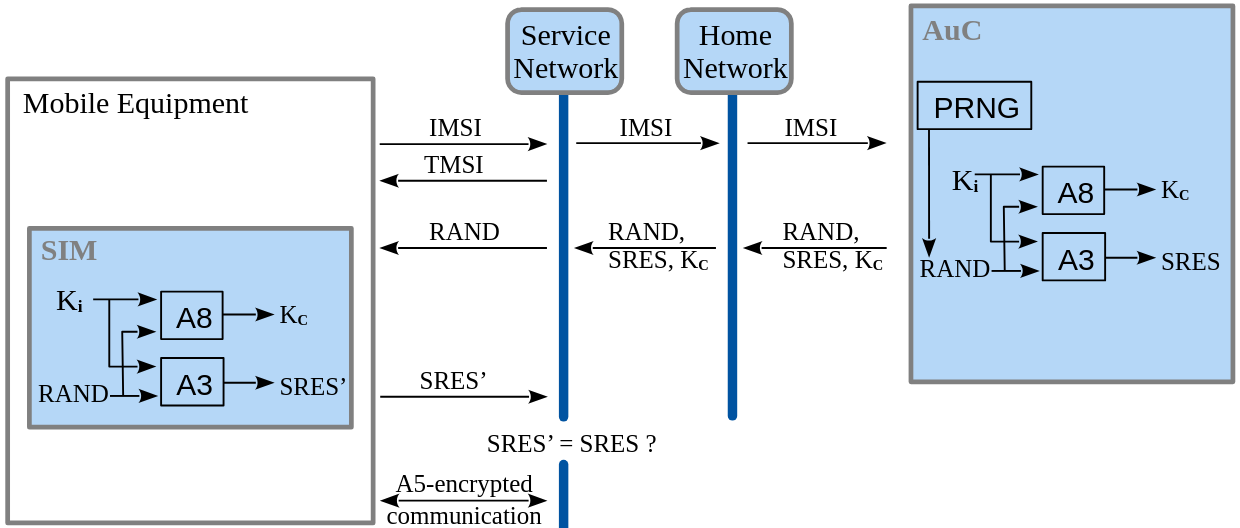
\includegraphics[width=0.9\columnwidth]{Resources/gsm_auth.png} % Adjust width and path
\begin{itemize}
    \item The \textbf{Service Network} sends a \textbf{RAND} (random challenge) to the Mobile Equipment (ME).
    \item The SIM card computes:
    \begin{itemize}
        \item \textbf{SRES'}: The signed response, using the authentication algorithm A3 and the subscriber key (\(K_i\)).
        \item \textbf{\(K_c\)}: The session key for encryption, generated using algorithm A8 and \(K_i\).
    \end{itemize}
    \item The \textbf{Authentication Center (AuC)} in the Home Network performs the same computations (using \(K_i\) stored in its database) to generate \textbf{SRES}.
    \item The network compares the \textbf{SRES'} received from the ME with its own \textbf{SRES}. If they match, authentication is successful.
    \item Communication is encrypted using the generated \textbf{\(K_c\)} and the A5 stream cipher.
\end{itemize}
\textbf{Glossary:}
\begin{itemize}
    \item \textbf{IMSI:} International Mobile Subscriber Identity, a unique identifier for the subscriber.
    \item \textbf{TMSI:} Temporary Mobile Subscriber Identity, a pseudonym for the IMSI used for privacy.
    \item \textbf{\(K_i\):} Subscriber key, stored on the SIM and at the network's Authentication Center.
    \item \textbf{PRNG:} Pseudo-Random Number Generator, used to generate the RAND challenge.
\end{itemize}

\subsubsection{IMSI Catcher}
\begin{itemize}
    \item \textbf{Man-in-the-Middle attack:}
    \begin{itemize}
        \item \textbf{IMSI Catcher:} A device (e.g., “Stingray”) impersonates a legitimate Base Station to intercept communications.
        \item \textbf{Step-by-step process:}
        \begin{itemize}
            \item The IMSI catcher pretends to be a Base Station with a strong signal, forcing nearby mobile devices to connect.
            \item The mobile device sends its IMSI (International Mobile Subscriber Identity) to the catcher for authentication.
            \item The IMSI catcher forwards authentication requests to the real Base Station, acting as a mobile phone.
            \item Once connected, the IMSI catcher can:
            \begin{itemize}
                \item Intercept data and voice traffic.
                \item Disable encryption by negotiating an unencrypted or weaker cipher mode.
                \item Track users by capturing their IMSI or location data.
            \end{itemize}
        \end{itemize}
        \item This method exploits the lack of mutual authentication in GSM networks (i.e., the mobile phone does not verify the Base Station's authenticity).
    \end{itemize}
\end{itemize}

\subsection{UMTS}
\subsubsection{Security Improvements}
\begin{itemize}
    \item \textbf{3GPP} (\emph{3rd Generation Partnership Project})
    \begin{itemize}
        \item Responsible for specifications, including issuing \emph{5G standards}.
    \end{itemize}
    \item \textbf{“Old” GSM SIM cards} can still be used:
    \begin{itemize}
        \item Backwards compatibility supports GSM authentication protocols.
    \end{itemize}
    \item \textbf{Circuit and Packet Switching:} Both methods available for communication.
    \item \textbf{Improved Crypto:}
    \begin{itemize}
        \item \emph{3GPP publishes cryptographic algorithms.}
        \item Encryption is applied \textbf{not only on the air}, enhancing security.
    \end{itemize}
    \item \textbf{New Encryption Algorithms:}
    \begin{itemize}
        \item Initially introduced \textbf{KASUMI}, used for encryption and CBC-MAC.
        \item Later replaced by more secure algorithms, as \textbf{KASUMI was broken}.
    \end{itemize}
    \item \textbf{Mutual Authentication:} 
    \begin{itemize}
        \item \emph{Both user and network authenticate each other (not mandatory).}
    \end{itemize}
    \item \textbf{Main Problems:}
    \begin{itemize}
        \item Backwards compatibility creates vulnerabilities.
        \item \emph{Fallback to GSM weakens overall security.}
    \end{itemize}
\end{itemize}

\subsection{LTE- Long Term Evolution}
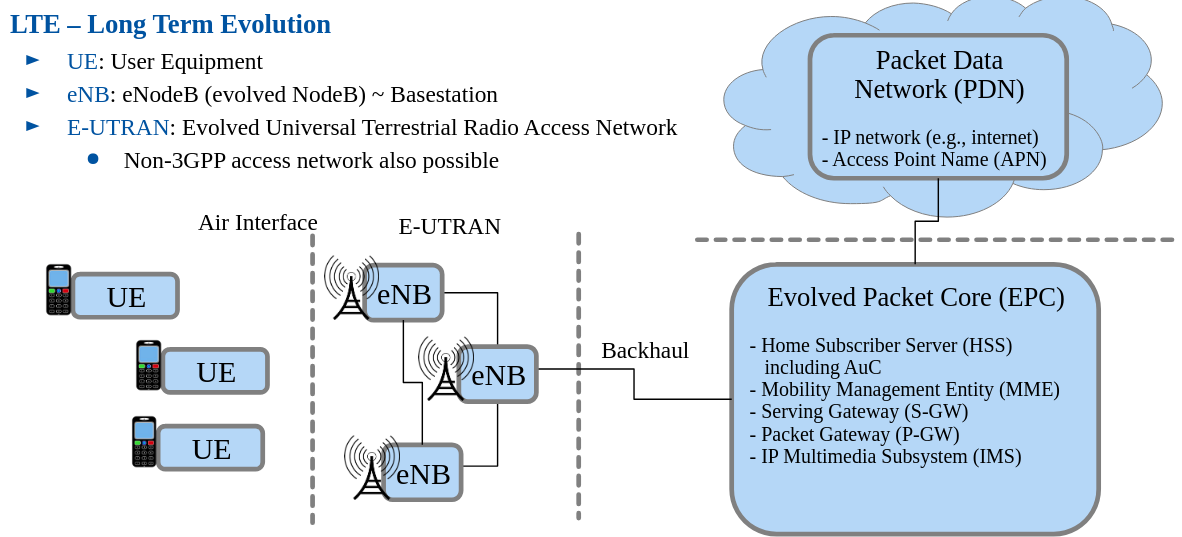
\includegraphics[width=1\columnwidth]{Resources/lte.png}
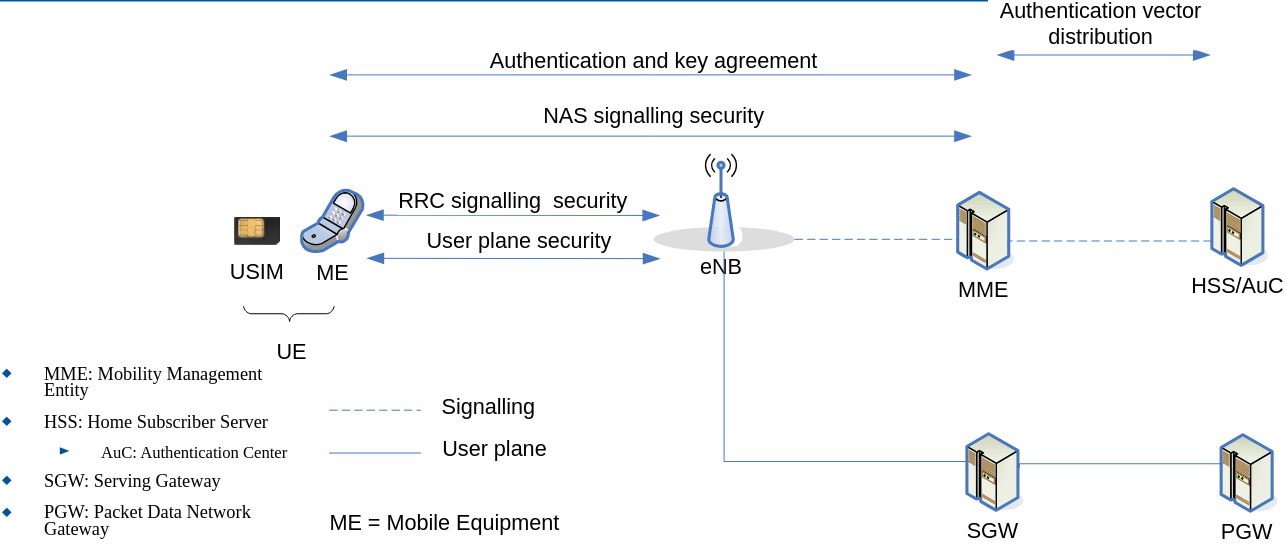
\includegraphics[width=1\columnwidth]{Resources/lte2.png}

\subsubsection{Protocol Stack}
\subsubsection{LTE Protocol Stack}
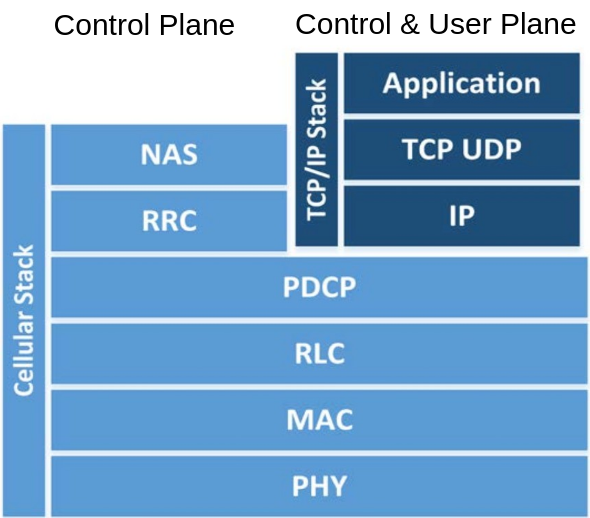
\includegraphics[width=0.3\columnwidth]{Resources/lte_protocols.png} % Adjust width and path
\begin{itemize}
    \item \textbf{Control Plane:}
    \begin{itemize}
        \item Handles signaling, network resource management, and routing.
        \item Ensures communication setup and maintenance.
    \end{itemize}
    \item \textbf{User Plane:}
    \begin{itemize}
        \item Responsible for transferring user data (e.g., voice, video, and application data).
        \item Integrates directly with applications via the TCP/IP stack.
    \end{itemize}
    \item \textbf{Key Protocols (Cellular Stack):}
    \begin{itemize}
        \item \textbf{NAS (Non-Access Stratum):}
        \begin{itemize}
            \item Manages mobility and session-related signaling between the UE and the core network (e.g., authentication, location updates).
        \end{itemize}
        \item \textbf{RRC (Radio Resource Control):}
        \begin{itemize}
            \item Handles signaling at the radio level, such as connection setup, handovers, and state management.
        \end{itemize}
        \item \textbf{PDCP (Packet Data Convergence Protocol):}
        \begin{itemize}
            \item Provides header compression, encryption, and integrity protection for user and control plane data.
        \end{itemize}
        \item \textbf{RLC (Radio Link Control):}
        \begin{itemize}
            \item Ensures data reliability through retransmissions and error correction.
        \end{itemize}
        \item \textbf{MAC (Medium Access Control):}
        \begin{itemize}
            \item Manages resource allocation and data multiplexing for multiple UEs.
        \end{itemize}
        \item \textbf{PHY (Physical Layer):}
        \begin{itemize}
            \item Deals with the actual transmission of radio signals over the air interface.
        \end{itemize}
    \end{itemize}
    \item \textbf{Integration with Applications:}
    \begin{itemize}
        \item The LTE stack works alongside the TCP/IP stack for application-level data transfer:
        \begin{itemize}
            \item Application protocols (e.g., HTTP, VoIP) run on top of \textbf{TCP/UDP}.
            \item \textbf{IP} ensures routing and addressing across networks.
            \item PDCP compresses and encrypts packets before passing them to the lower layers for radio transmission.
        \end{itemize}
    \end{itemize}
\end{itemize}
\subsubsection{Authentication}
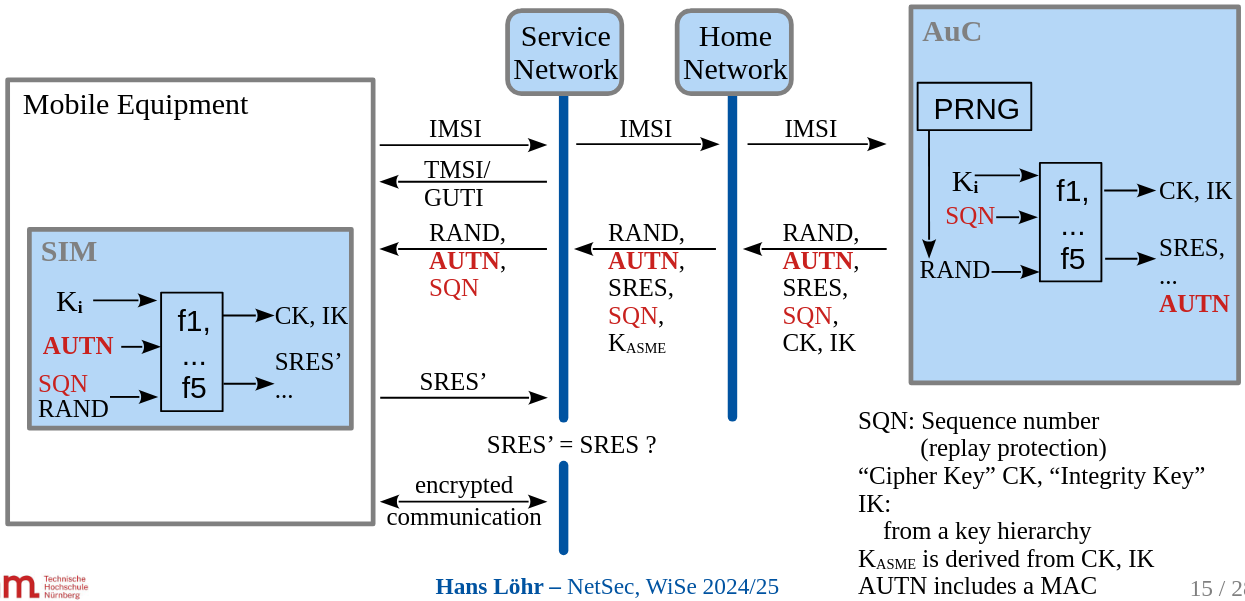
\includegraphics[width=0.8\columnwidth]{Resources/lte_auth.png} 
\begin{itemize}
    \item \textbf{Authentication Process:}
    \begin{itemize}
        \item The \textbf{Home Network} sends a random challenge (\textbf{RAND}), an authentication token (\textbf{AUTN}), and a sequence number (\textbf{SQN}) to the \textbf{Mobile Equipment (ME)}.
        \item The \textbf{SIM card} in the ME uses the \textbf{subscriber key (\(K_i\))} and predefined functions (\(f1, f2, \ldots, f5\)) to compute:
        \begin{itemize}
            \item \textbf{SRES':} Signed response for authentication.
            \item \textbf{CK:} Cipher key for encryption.
            \item \textbf{IK:} Integrity key for data integrity.
        \end{itemize}
        \item The \textbf{ME} sends \textbf{SRES'} back to the network for verification.
        \item If \textbf{SRES'} matches the expected \textbf{SRES}, authentication is successful, and encrypted communication begins.
    \end{itemize}

    \item \textbf{Acronyms:}
    \begin{itemize}
        \item \textbf{RAND:} Random number used for the challenge.
        \item \textbf{AUTN:} Authentication token, includes a MAC (Message Authentication Code).
        \item \textbf{SQN:} Sequence number for replay protection.
        \item \textbf{\(K_i\):} Subscriber key shared between SIM and the Home Network.
        \item \textbf{CK:} Cipher key, used for encrypting data.
        \item \textbf{IK:} Integrity key, used for ensuring data integrity.
        \item \textbf{K\(_{\text{ASME}}\):} Key derived from \textbf{CK} and \textbf{IK}, used for session management.
    \end{itemize}

    \item \textbf{Security Features:}
    \begin{itemize}
        \item Protects against replay attacks using \textbf{SQN}.
        \item Ensures mutual authentication with \textbf{AUTN} and \textbf{SRES}.
        \item Enables encrypted communication using \textbf{CK}.
    \end{itemize}
\end{itemize}

\subsubsection{Crypto Algorithms}
\begin{itemize}
    \item \textbf{Authentication Algorithms:}
    \begin{itemize}
        \item \(f1, f2\): Message Authentication Codes (MACs), inherited from UMTS.
        \item Operator-specific (\textbf{MNO-dependent}); 3GPP recommends AES-based algorithms.
    \end{itemize}

    \item \textbf{Key Generation Algorithms (Key Derivation):}
    \begin{itemize}
        \item \(f3, f4, f5\): Used for deriving keys (e.g., \(K_c, K_i\)), also inherited from UMTS.
        \item Operator-specific (\textbf{MNO-dependent}); 3GPP recommends AES-based algorithms.
    \end{itemize}

    \item \textbf{Encryption Algorithms:}
    \begin{itemize}
        \item \textbf{EEA0:} "Null cipher" (no encryption).
        \item \textbf{128-EEA1:} SNOW 3G (stream cipher).
        \item \textbf{128-EEA2:} AES-based encryption algorithm (strong and widely used).
        \item \textbf{128-EEA3:} ZUC (Chinese stream cipher).
    \end{itemize}

    \item \textbf{Integrity Algorithms (EIA):}
    \begin{itemize}
        \item Similar to encryption, used to ensure data integrity during transmission.
    \end{itemize}
\end{itemize}

\subsubsection{Privacy}
\begin{itemize}
    \item \textbf{Fact:} Mobile Network Operators (MNOs) can always track their users (this is by design).
    \item \textbf{Additional Problem:} Eavesdropping on radio communication.
    \begin{itemize}
        \item \textbf{IMSI:} A unique identifier for a user:
        \begin{itemize}
            \item \textbf{GSM:} Used by the UE only when no \textbf{TMSI} is available.
            \item \textbf{LTE:} \textbf{IMSI} replaced by \textbf{GUTI} (Globally Unique Temporary Identifier).
        \end{itemize}
        \item \textbf{TMSI/GUTI}:
        \begin{itemize}
            \item Can (and should) be \textbf{updated frequently} to avoid tracking by third parties.
            \item Changes must be \textbf{unpredictable} to prevent tracking or identification.
        \end{itemize}
        \item Research findings:
        \begin{itemize}
            \item 19 out of 28 MNOs used \textbf{very simple, predictable patterns}, such as monotonic counters.
            \item Earlier research found \textbf{no or very rare changes}, allowing tracking.
        \end{itemize}
    \end{itemize}
\end{itemize}

\subsubsection{LTE Proximity Services (ProSe)}
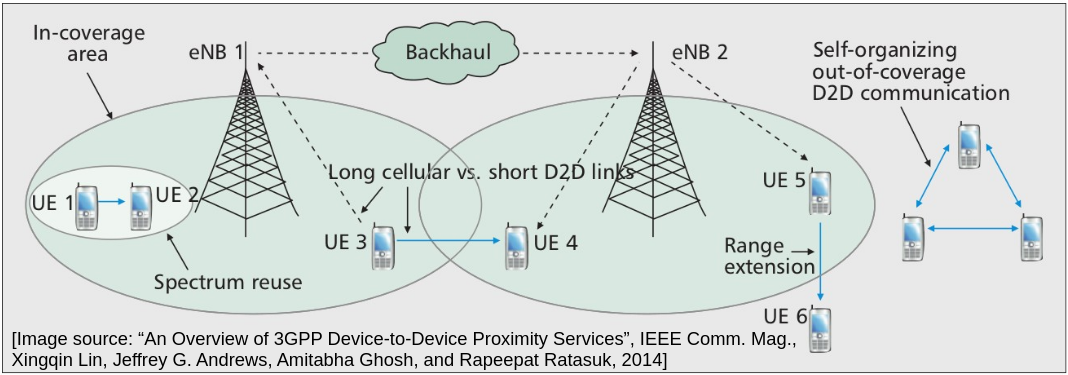
\includegraphics[width=0.7\columnwidth]{Resources/prose.png} 
\begin{itemize}
    \item \textbf{ProSe:} Cellular Device-to-Device (D2D) Communication
    \begin{itemize}
        \item Enables communication between devices directly, bypassing base stations.
        \item Can operate \textbf{with or without network coverage.}
        \item Commonly used in \textbf{public safety networks}, such as emergencies or disasters.
        \item \textbf{Applications:}
        \begin{itemize}
            \item Peer-to-peer applications.
            \item Location-based services.
            \item Range extension through device relays.
        \end{itemize}
    \end{itemize}

    \item \textbf{Control Modes:}\\
    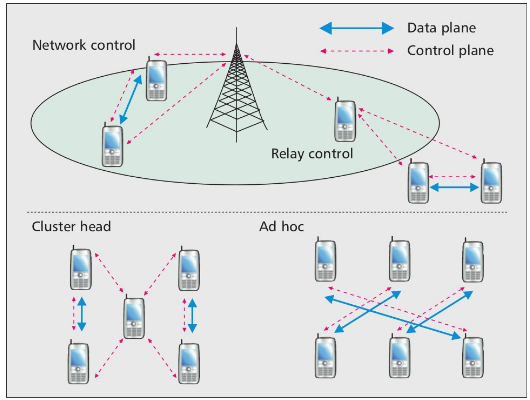
\includegraphics[width=0.5\columnwidth]{Resources/prose2.png} 
    \begin{itemize}
        \item \textbf{Network-Controlled Mode:}
        \begin{itemize}
            \item ProSe communication is managed via the LTE network for reliability and resource allocation.
        \end{itemize}
        \item \textbf{Cluster Head Mode:}
        \begin{itemize}
            \item A device (cluster head) acts as a local coordinator for nearby devices.
            \item Manages intra-cluster communication and relays data to the LTE network or other clusters.
        \end{itemize}
        \item \textbf{Ad Hoc Mode:}
        \begin{itemize}
            \item Devices communicate directly without centralized control.
            \item Suitable for completely out-of-coverage scenarios.
        \end{itemize}
    \end{itemize}

    \item \textbf{Key Management:}
    \begin{itemize}
        \item \textbf{Authorization:} User Equipment (UE) must be authorized unless pre-configured on the USIM.
        \item \textbf{MIKEY (Multimedia Internet Keying):}
        \begin{itemize}
            \item Used for VoIP key exchange.
            \item Supports different modes (e.g., pre-shared keys or PKI-based).
        \end{itemize}
        \item \textbf{Key Hierarchy:}
        \begin{itemize}
            \item ProSe MIKEY Key (PMK) → Temporary ProSe Group Key (PGK).
            \item PGK → ProSe Traffic Key (PTK) → ProSe Encryption Key (PEK).
        \end{itemize}
    \end{itemize}
\end{itemize}

\subsection{5G: The 5\textsuperscript{th} Generation Mobile Network}
\begin{itemize}
    \item \textbf{5G:} Represents the next and current generation of mobile networks.
    \item \textbf{Deployment:} Has already started, though some specifications are still evolving.
    \item \textbf{Performance:} 
    \begin{itemize}
        \item Much faster than 4G.
        \item Provides significantly lower latency and higher reliability.
    \end{itemize}
    \item \textbf{Advancements:}
    \begin{itemize}
        \item Builds on software-defined networking principles, initiated with LTE.
        \item Includes advanced \textbf{Quality-of-Service (QoS)} features.
    \end{itemize}
    \item \textbf{New Application Scenarios:}
    \begin{itemize}
        \item \textbf{Industry 4.0:} Automation and IoT for manufacturing and logistics.
        \item \textbf{Device-to-Device Communication:} Key for vehicular networks and ProSe.
        \item \textbf{Private Networks:} Operated by non-traditional operators, such as manufacturing industries.
    \end{itemize}
\end{itemize}

\subsubsection{5G Security: Relevant Entities (Functions)}
\begin{itemize}
    \item \textbf{AMF (Access and Mobility Management Function):} 
    Manages device access and mobility in the Serving Network.

    \item \textbf{SEAF (Security Anchor Functionality):} 
    Handles initial authentication and acts as the anchor point for security in the Serving Network.

    \item \textbf{AUSF (Authentication Server Function):} 
    Processes authentication in the Home Network, replacing the HSS from LTE.

    \item \textbf{ARPF (Authentication Credential Repository and Processing Function):} 
    Stores and processes authentication keys, like the AuC in LTE.

    \item \textbf{SEPP (Security Edge Protection Proxy):} 
    Secures inter-operator communication (e.g., roaming) by protecting signaling messages exchanged between networks.\\
    \\
\end{itemize}
\begin{itemize}
    \item \textbf{IMSI → SUPI (Subscription Permanent Identifier):}
    \begin{itemize}
        \item \textbf{SUPI:} Replaces IMSI and is never transmitted unencrypted over the air.
        \item \textbf{SUCI (Subscription Concealed Identifier):}
        \begin{itemize}
            \item SUPI is encrypted using the network's public key to create SUCI for secure transmission.
        \end{itemize}
        \item \textbf{TMSI → 5G-S-TMSI:} Mandatory to change after paging (e.g., during basestation handover).
        \item \textbf{GUTI → 5G-GUTI:} Requirements for dynamic GUTI changes to improve privacy.
    \end{itemize}

    \item \textbf{Authentication (AKA):}
    \begin{itemize}
        \item Protocol improvements to better protect security features and enhance user privacy.
    \end{itemize}

    \item \textbf{IMSI Catcher Detection:}
    \begin{itemize}
        \item \textbf{Measurement Reports:} Enable network-based and UE-assisted detection.
        \item Makes IMSI/SUCI catchers harder to deploy without being detected.
    \end{itemize}

    \item \textbf{Security in 5G Standalone Mode:}
    \begin{itemize}
        \item Many advanced features are available only in 5G "Standalone" mode.
        \item Current usage is mainly \textbf{5G NSA (Non-Standalone)} for cooperation with 4G (LTE).
    \end{itemize}
\end{itemize}

\subsubsection{Authentication and Key Agreement}
\begin{itemize}
    \item \textbf{Authentication Options:}
    \begin{itemize}
        \item \textbf{EAP-AKA'}:
        \begin{itemize}
            \item Defined in RFC5448.
            \item Based on pre-shared keys.
            \item Fits into the EAP (Extensible Authentication Protocol) framework.
        \end{itemize}
        \item \textbf{5G AKA}:
        \begin{itemize}
            \item Derived from LTE AKA for backward compatibility.
        \end{itemize}
    \end{itemize}

    \item \textbf{Privacy Concerns:}
    \begin{itemize}
        \item Flaws in 5G AKA found via formal protocol analysis:
        \begin{itemize}
            \item \textit{David Basin et al., "A Formal Analysis of 5G Authentication", ACM CCS 2018}.
        \end{itemize}
        \item Practical attacks require targeting specific users:
        \begin{itemize}
            \item \textit{Chlosta, Rupprecht, Pöpper, Holz, "5G SUCI-Catchers: Still catching them all?", ACM WiSec 2021}.
        \end{itemize}
    \end{itemize}
\end{itemize}

\subsubsection{Service-Based Interfaces}
\begin{itemize}
    \item \textbf{Network Operators and 3rd Parties Offering "Services":}
    \begin{itemize}
        \item \textbf{Network Functions (NF):} Core network features exposed as services.
        \item \textbf{Other Services:} Additional functionalities provided by the network.
        \item \textbf{TLS Support:} Ensures secure communication between entities.
        \item \textbf{OAuth 2.0-based Authorization:} Allows secure access control using access tokens.
    \end{itemize}

    \item \textbf{Network Slices:}
    \begin{itemize}
        \item Provides virtualized and isolated network partitions with specific \textbf{QoS (Quality of Service)} properties.
        \item Uses \textbf{EAP-based Authorization} for access control.
    \end{itemize}
\end{itemize}

\section{Firewalls, Intrusion Detection and Prevention}
\subsection{Firewalls}
\begin{itemize}
  \item Firewalls separate networks
    \begin{itemize}
      \item Restricts traffic: enforces policy
      \item Logging
      \item Implemented in SW and/or HW)
    \end{itemize}
\end{itemize}

\subsubsection{Packet Filtering}
\begin{itemize}
    \item \textbf{Packet filtering firewalls:}
    \begin{itemize}
        \item Policies defined by filtering rules (source, destination, port, protocol, etc.).
        \item Rules decide actions: accept, block, log, or modify packets.
        \item Advanced filters can modify packets (e.g., NAT or port translation).
    \end{itemize}

    \item \textbf{Advantages:}
    \begin{itemize}
        \item Cheap, widely available, and efficient.
        \item Examples: Linux \texttt{netfilter}, Windows firewall.
        \item Simple implementation; no modification to applications required.
    \end{itemize}

    \item \textbf{Limitations:}
    \begin{itemize}
        \item Susceptible to IP and port spoofing attacks.
        \item Rules limited to individual packets and lack comprehensive state awareness.
        \item Cannot enforce application-specific filtering; lacks deeper protocol knowledge.
        \item Usually not capable of rejecting specific packets within a particular application session.
    \end{itemize}

    \item \textbf{Niche Aspects:}
    \begin{itemize}
        \item Filters can reject IP spoofing by blocking packets from internal addresses arriving at external interfaces.
        \item Access control by ports can restrict services to specific source addresses (e.g., SMTP limited to internal IPs).
        \item Can filter based on packet type (TCP, UDP) or flags (e.g., SYN for connection establishment).
    \end{itemize}
\end{itemize}

\subsubsection{Connection Tracking and Stateful Firewalls}
\begin{itemize}
    \item \textbf{Connection Tracking:}
    \begin{itemize}
        \item Tracks packets belonging to the same logical "connection" (not limited to TCP).
        \item Examples:
        \begin{itemize}
            \item UDP-based connections (e.g., DTLS).
            \item DNS requests/responses and ICMP echo/replies.
        \end{itemize}
        \item Supports protocols with separate control and data connections (e.g., active FTP).
        \item Enables NAT functionality by rewriting addresses for complex protocols.
    \end{itemize}
    
    \item \textbf{Stateful Firewalls:}
    \begin{itemize}
        \item Maintain state information about active connections.
        \item Rules can dynamically adapt based on connection states (e.g., allow replies to outgoing requests).
    \end{itemize}
\end{itemize}

\subsubsection{Linux Firewall: Netfilter}
Netfilter, part of the Linux kernel, is a framework for packet filtering and network address translation (NAT). It operates using a series of hooks in the network stack where rules, organized into \textbf{tables} and \textbf{chains}, are applied.
\paragraph{Chains and Their Functions:}
\begin{itemize}
    \item \textbf{Input Chain:} Handles packets destined for the local system (e.g., filtering SSH traffic).
    \item \textbf{Output Chain:} Manages packets generated locally and leaving the system (e.g., limiting outgoing ICMP traffic).
    \item \textbf{Forward Chain:} Processes packets passing through the system but not destined for it (e.g., traffic routing in a gateway).
    \item \textbf{Prerouting Chain:} Alters incoming packets before routing decisions (e.g., DNAT for port redirection).
    \item \textbf{Postrouting Chain:} Alters outgoing packets after routing decisions (e.g., SNAT for source IP modification).
\end{itemize}
\paragraph{Key Components:}
\begin{itemize}
    \item \textbf{Tables:} Contain chains for specific tasks:
    \begin{itemize}
        \item \textbf{Filter Table:} Default table for packet filtering (Input, Output, Forward chains).
        \item \textbf{NAT Table:} Used for network address translation (Prerouting, Postrouting chains).
        \item \textbf{Mangle Table:} For modifying packet headers.
    \end{itemize}
    \item \textbf{Tools:}
    \begin{itemize}
        \item \texttt{iptables}: Legacy tool for managing rules.
        \item \texttt{nftables}: Modern replacement offering simplified syntax and better performance.
    \end{itemize}
\end{itemize}
\paragraph{Use Case Example:}
A packet enters the system through the \textbf{Prerouting Chain}, is routed to the appropriate interface (via \textbf{Forward Chain} if being forwarded or \textbf{Input Chain} if destined locally), and exits through the \textbf{Postrouting Chain} after necessary modifications.
Netfilter’s modularity and flexibility make it a powerful tool for managing network traffic.

\subsubsection{Application-Level Gateways}
An \textbf{Application-Level Gateway (ALG)} acts as an intermediary between clients and applications, offering fine-grained control and monitoring of traffic specific to application protocols. It provides a specialized interface tailored for applications, such as SMTP or HTTP, allowing for filtering, logging, and user profiling at the application layer.
\paragraph{Functionality:}
\begin{itemize}
    \item \textbf{Connection Handling:} Clients connect to the gateway, which filters and analyzes the traffic before forwarding it to the application server.
    \item \textbf{Protocol Awareness:} Equipped with detailed knowledge of application-specific protocols, enabling in-depth traffic inspection and filtering.
    \item \textbf{State Management:} Tracks the state of connections or application data to enforce security or logging policies effectively.
\end{itemize}
\begin{itemize}
    \item In-depth analysis and traffic filtering based on application logic.
    \item Enables user profiling, attack detection, and intrusion prevention.
    \item Provides application-specific caching and potential for secure communication.
    \item App extensions for additional features, such as authentication, without modifying the original application.
\end{itemize}
\paragraph{Limitations:}
\begin{itemize}
    \item \textbf{Performance Overhead:} The inspection and filtering process can reduce throughput.
    \item \textbf{Maintenance Effort:} Requires frequent updates to stay compatible with evolving application protocols.
    \item \textbf{Limited Scope:} Only supports predefined applications, limiting flexibility in heterogeneous environments.
\end{itemize}
\paragraph{Use Case:}
ALGs are frequently employed in enterprise environments for managing email servers (e.g., SMTP gateways) or for secure access to critical applications by acting as a filter and logging interface for external traffic.

\subsubsection{Proxy Firewalls}
Proxy firewalls act as a generic proxy on the transport layer, enabling advanced traffic control and enhancing communication security.
\paragraph{Key Features:}
\begin{itemize}
    \item \textbf{Connection State Tracking:} Monitors and manages the state of connections.
    \item \textbf{Authentication and Security:} Adds user authentication and communication security.
    \begin{itemize}
        \item Frequently used in corporate environments:
        \begin{itemize}
            \item Outgoing traffic is routed only via the proxy.
            \item User authentication is required before access.
            \item Only specific ports or applications are allowed.
        \end{itemize}
    \end{itemize}
    \item \textbf{Flexibility:} Can extend functionality toward application-level filtering (e.g., web proxies or caches).
\end{itemize}
\paragraph{Comparison to Application-Level Gateways:}
\begin{itemize}
    \item Proxy firewalls are more general than application-level gateways.
    \item The distinction between proxy firewalls and application gateways is not always clear.
\end{itemize}

\subsubsection*{Firewall Architectures: Dual-Homed Firewall vs. DMZ}
\begin{itemize}
    \item \textbf{Dual-Homed Firewall:}\\
    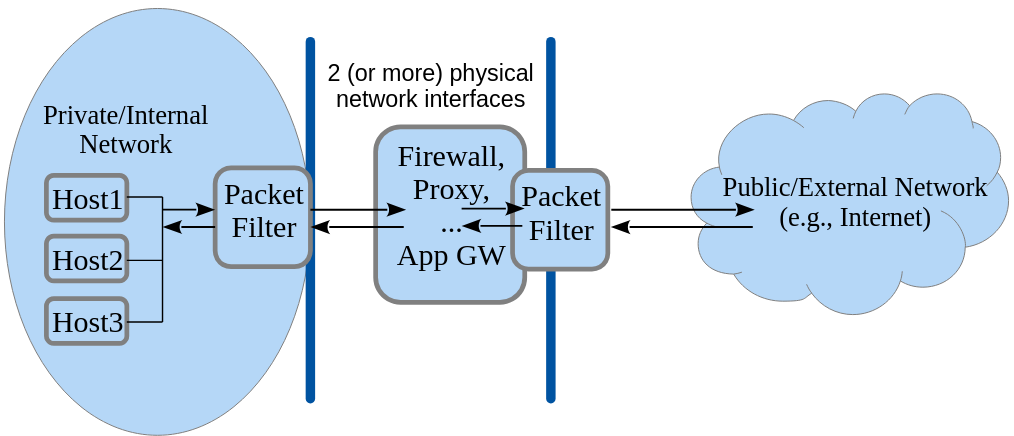
\includegraphics[width=0.7\columnwidth]{Resources/dual-homed.png} 
    \begin{itemize}
        \item \textit{Concept:} Firewall with two interfaces separating internal and external networks.
        \item \textit{Operation:} Traffic flows through the firewall, using packet filters or proxies for mediation.
        \item \textit{Advantages:}
        \begin{itemize}
            \item Strong physical isolation.
            \item Centralized traffic control.
            \item Flexible integration of security mechanisms.
        \end{itemize}
        \item \textit{Disadvantages:}
        \begin{itemize}
            \item Requires additional hardware resources.
            \item Limited scalability for complex networks.
        \end{itemize}
        \item \textit{Use Cases:} Suitable for small/medium networks needing strict isolation.
    \end{itemize}

    \item \textbf{Demilitarized Zone (DMZ):}\\
    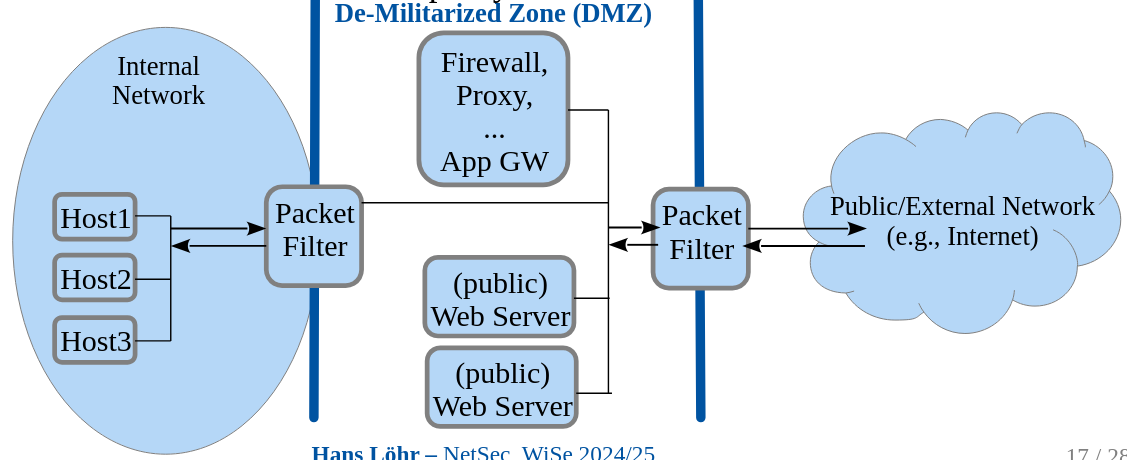
\includegraphics[width=0.8\columnwidth]{Resources/dmz.png} 
    \begin{itemize}
        \item \textit{Concept:} Segregated network zone for public-facing services (e.g., web servers).
        \item \textit{Operation:} Packet filters manage traffic to/from DMZ, preventing direct internal access.
        \item \textit{Advantages:}
        \begin{itemize}
            \item Protects internal networks from compromised public-facing services.
            \item Granular traffic control for specific services.
            \item Limits exposure of internal systems.
        \end{itemize}
        \item \textit{Disadvantages:}
        \begin{itemize}
            \item Adds configuration and maintenance complexity.
        \end{itemize}
        \item \textit{Use Cases:} Ideal for hosting public services (e.g., web hosting, e-commerce).
    \end{itemize}

    \item \textbf{Key Differences:}
    \begin{itemize}
        \item Dual-Homed focuses on isolation, while DMZ separates public services from internal systems.
        \item DMZ adds a dedicated network segment for external-facing servers.
    \end{itemize}
\end{itemize}

\subsection{Intrusion Detection and Prevention System (IDPS)}
\begin{itemize}
    \item \textbf{Intrusion Detection Systems (IDSs):}
    \begin{itemize}
        \item Detect attempts to attack or intrusions.
        \item Focused on monitoring and logging suspicious activities.
    \end{itemize}
    \item \textbf{Prevention:}
    \begin{itemize}
        \item React to detected intrusions to prevent successful attacks.
        \item Goal: Stop attacks in progress by blocking or responding.
    \end{itemize}
    \item \textbf{IDPS = IDS + Prevention:} Combines detection and prevention to ensure proactive and reactive defense mechanisms.
    \item \textbf{Historical Work:}
    \begin{itemize}
        \item James Anderson: \emph{Computer Security Threat Monitoring and Surveillance} (1980).
        \item Dorothy Denning: \emph{An Intrusion Detection Model} (1987).
    \end{itemize}
\end{itemize}
\paragraph{Why Use IDPS?}
\begin{itemize}
    \item Identify incidents effectively.
    \item Support incident response to minimize damage.
    \item Identify gaps in security policy and practices.
    \item Deter insiders from violating policies.
\end{itemize}

\subsubsection{IDPS Functionality (High-Level)}
\begin{itemize}
    \item \textbf{Record Events:}
    \begin{itemize}
        \item Logging and accounting for detected activities.
        \item Observations useful for detecting and analyzing incidents.
        \item Integration with Security Information and Event Management (SIEM) systems.
    \end{itemize}
    \item \textbf{Notify Administrators:}
    \begin{itemize}
        \item Alert administrators to take appropriate action.
    \end{itemize}
    \item \textbf{Produce Reports:}
    \begin{itemize}
        \item Summarize activities and detected threats for analysis.
    \end{itemize}
    \item \textbf{Automated First-Level Reaction:}
    \begin{itemize}
        \item Stop attacks or intrusion attempts automatically.
        \item Dynamically change the security environment, e.g., reconfigure firewalls.
    \end{itemize}
\end{itemize}

\subsubsection{Intrusion Detection Model (Denning, 1987)}
\begin{itemize}
    \item \textbf{Components:}
    \begin{itemize}
        \item \textbf{Subjects:} Entities initiating actions.
        \item \textbf{Objects:} Resources being accessed or affected.
        \item \textbf{Audit Records:} Logs of subject actions for monitoring.
        \item \textbf{Profiles:} Behavioral characterizations based on metrics.
        \item \textbf{Anomaly Records:} Highlight abnormal activities.
        \item \textbf{Activity Rules:} Define responses to anomalies (e.g., profile updates, intrusion reporting).
    \end{itemize}
    \item \textbf{Metrics:}
    \begin{itemize}
        \item Event Counters
        \item Interval Timers
        \item Resource Measures
    \end{itemize}
    \item \textbf{Models:}
    \begin{itemize}
        \item \textbf{Statistical Models:} Identify statistical anomalies.
        \begin{itemize}
            \item Mean and Standard Deviation Model
            \item Multivariate Correlation Model
            \item Markov Process Model
            \item Time Series Model
        \end{itemize}
        \item \textbf{Operational Models:} Compare metrics against predefined thresholds.
        \item \textbf{Modern Approaches:} Incorporate Machine Learning/AI for advanced anomaly detection.
    \end{itemize}
\end{itemize}

\subsubsection{Types of IDPS}
\begin{itemize}
    \item \textbf{Network-Based Intrusion Detection System (NIDS):}
    \begin{itemize}
        \item Monitors and analyzes network traffic.
        \item Often integrated with firewalls (tightly or loosely).
        \item Includes specialized Wireless IDPS for wireless networks.
        \item Incorporates Network Behavior Analysis (NBA) for deeper traffic insights.
    \end{itemize}
    \item \textbf{Host-Based Intrusion Detection System (HIDS):}
    \begin{itemize}
        \item Monitors activity on a specific host (server or end-user device).
        \item Analyzes system and application logs, network activity, running processes, and system calls.
        \item Tracks file accesses and configuration changes for anomaly detection.
    \end{itemize}
\end{itemize}

\subsubsection{IDPS Architecture}
\begin{itemize}
    \item \textbf{Sensors (Agents):} Monitor and analyze activity.
    \item \textbf{IDPS Management Server:} Collects information from sensors and manages them.
    \item \textbf{Database:} Serves as a repository for audit records.
    \item \textbf{Admin Console:} Provides a user interface for administrators.
\end{itemize}

\subsubsection{Detection Methodologies: Categorization}
\begin{itemize}
    \item \textbf{Signature-Based Intrusion Detection}
    \begin{itemize}
        \item Uses fixed patterns to identify \textit{known threats} (e.g., hash values of malware).
        \item Limited to known threats and can be evaded by intelligent attackers.
    \end{itemize}
    \item \textbf{Anomaly-Based Intrusion Detection}
    \begin{itemize}
        \item Detects previously unknown threats by modeling normal/abnormal behavior.
        \item Requires a \textit{training/learning phase} for data collection and profiling.
        \item Often uses Machine Learning or AI; main focus of current research.
    \end{itemize}
    \item \textbf{Specification-Based Intrusion Detection (Stateful Protocol Analysis)}
    \begin{itemize}
        \item Compares observations to models/specifications of legitimate behavior.
        \item Can be integrated into application-level gateways.
    \end{itemize}
\end{itemize}

\subsection{Summary}
\begin{itemize}
    \item \textbf{Firewalls}
    \begin{itemize}
        \item Essential building block for network security.
        \item Alone cannot effectively prevent attacks.
        \item Various types:
        \begin{itemize}
            \item Packet filters.
            \item Application-level gateways/proxies.
        \end{itemize}
        \item Example: Linux firewall (netfilter, iptables/nftables).
    \end{itemize}
    \item \textbf{Intrusion Detection and Prevention Systems (IDPS)}
    \begin{itemize}
        \item Detect and prevent intrusion attempts.
        \item Types:
        \begin{itemize}
            \item Host-based vs. Network-based IDPS.
        \end{itemize}
        \item Detection methodologies:
        \begin{itemize}
            \item Signature-based.
            \item Behavior-based (e.g., anomaly detection).
        \end{itemize}
        \item Specialized IDPS for specific systems (e.g., industrial automation, vehicle networks).
    \end{itemize}
\end{itemize}

\section{Border Gateway Protocol (BGP), Domain Name System (DNS)}
\subsection{Routing}
\begin{itemize}
    \item \textbf{Routing:} Finding the best path from source to destination.
    \begin{itemize}
        \item \textit{Internal routing:} Within a network or AS (Autonomous System).
        \item \textit{External routing:} Between networks or ASes.
        \item Different types of routing algorithms exist.
    \end{itemize}
    \item \textbf{Distance Vector Algorithms (e.g., Bellman-Ford):}
    \begin{itemize}
        \item Practical for networks of limited size $\Rightarrow$ used for internal routing.
    \end{itemize}
    \item \textbf{Link-State Algorithms (e.g., Dijkstra):}
    \begin{itemize}
        \item Computes the shortest path.
        \item Suitable for networks of limited size $\Rightarrow$ used for internal routing.
    \end{itemize}
    \item \textbf{Path-Vector Algorithms:}
    \begin{itemize}
        \item Advertises paths to reach destinations.
        \item Suitable for external routing between networks.
    \end{itemize}
\end{itemize}

\subsection{Border Gateway Protocol (BGP)}
\begin{itemize}
    \item \textbf{Border Gateway Protocol (BGP):}
    \begin{itemize}
        \item Originally specified in RFC 1105 (1989).
        \item Current version: BGP4 (RFC 4271, 2006).
    \end{itemize}
    \item \textbf{Border Routers:} Connect Autonomous Systems (AS).
    \item \textbf{External BGP (eBGP):}
    \begin{itemize}
        \item Operates between ASes.
        \item Uses Classless Inter-Domain Routing (CIDR) prefixes.
        \item Advertises:
        \begin{itemize}
            \item Routing prefixes for the router's own network.
            \item Prefixes from connected ASes (includes the \textit{AS path}).
        \end{itemize}
    \end{itemize}
    \item \textbf{Internal BGP (iBGP):}
    \begin{itemize}
        \item Operates within an AS.
        \item Used to propagate BGP information internally.
    \end{itemize}
\end{itemize}

\subsubsection{Internet Interconnection Ecosystem}
\begin{itemize}
    \item \textbf{Internet Exchange Points (IXP):}
    \begin{itemize}
        \item Locations where ISPs and ASes exchange traffic.
        \item Examples: DE-CIX, AMS-IX, N-IX.
    \end{itemize}
    \item \textbf{Connections between Autonomous Systems:}
    \begin{itemize}
        \item \textbf{Peering:}
        \begin{itemize}
            \item ASes agree to exchange traffic without charge.
            \item Typically between ASes of similar size.
        \end{itemize}
        \item \textbf{Transit:}
        \begin{itemize}
            \item One AS pays another for interconnection services.
        \end{itemize}
    \end{itemize}
    \item \textbf{Challenges:}
    \begin{itemize}
        \item Missing economic incentives to improve interconnection infrastructure.
    \end{itemize}
\end{itemize}

\subsubsection{Resilience and Security}
\begin{itemize}
    \item \textbf{Route Filtering:}
    \begin{itemize}
        \item Best practices: filter route announcements to limit accepted routes.
        \item Issues: not universally supported; mainly benefits others.
        \item Example: lack of IP spoofing packet filtering.
    \end{itemize}
    \item \textbf{Enormous Scale:}
    \begin{itemize}
        \item Hard to attack large portions of the internet due to diversity.
        \item Increasing centralization: few large players (e.g., Google, Akamai, Cloudflare).
    \end{itemize}
    \item \textbf{Missing Data and Metrics:}
    \begin{itemize}
        \item Lack of global transparency; commercial secrecy.
        \item Difficult to evaluate network interconnection resilience.
        \item Historically robust, but future concerns exist.
    \end{itemize}
    \item \textbf{Regulation:}
    \begin{itemize}
        \item Historically minimal.
        \item Country-dependent: some regulations harm free/open internet.
        \item Market concentration may require anti-trust regulation (e.g., oligopolies).
    \end{itemize}
    \item \textbf{Future:} Moving towards \textbf{BGPsec} for improved security.
\end{itemize}

\subsubsection{BGPsec: Simplified Overview}
\begin{itemize}
    \item \textbf{Definition:} BGPsec (RFC 8205, 2017) focuses on AS path validation.
    \item \textbf{Key Features:}
    \begin{itemize}
        \item Utilizes \textbf{Resource PKI (RPKI)} to certify which AS is responsible for specific IP prefixes.
        \item AS explicitly authorizes the next AS in the path to announce the route.
        \begin{itemize}
            \item BGP UPDATE message includes \texttt{AS\_PATH} (BGP) $\rightarrow$ \texttt{BGPsec\_PATH}.
            \item Each BGPsec-capable AS:
            \begin{itemize}
                \item Needs an RPKI certificate.
                \item Signs prefix and \texttt{BGPsec\_PATH} with its private key.
            \end{itemize}
            \item Recipient verifies all ASes on the path were explicitly authorized.
        \end{itemize}
    \end{itemize}
    \item \textbf{Issues:}
    \begin{itemize}
        \item Lack of incentives for ASes to support BGPsec.
        \item Cryptographic overhead may impact resilience (e.g., handling unsigned announcements during recovery).
        \item Preventing malicious ASes (with legitimate IPs) from injecting routes.
    \end{itemize}
\end{itemize}

\subsubsection{Summary}
\begin{itemize}
    \item \textbf{BGP seems fragile?}
    \begin{itemize}
        \item Easily disturbed by failures or attacks.
        \item \textbf{No global view:} Each AS has only local knowledge of its network and direct neighbors.
        \item Explicit contracts/partnerships only with direct neighbors.
        \item \textbf{Limited technical security:} Relies on trust, contracts, and decentralized motivation.
    \end{itemize}
    \item \textbf{Little is known about the internet interconnection ecosystem:}
    \begin{itemize}
        \item Lack of global view and detailed measurement data.
        \item Effects of incidents are unpredictable.
    \end{itemize}
    \item \textbf{BGP seems resilient?}
    \begin{itemize}
        \item Internet functions well despite limitations.
        \item Disaster recovery has been effective in the past.
    \end{itemize}
\end{itemize}

\subsection{DNS}
\begin{itemize}
    \item \textbf{DNS lookup retrieves a resource record:}
    \begin{itemize}
        \item \textbf{Types of records:}
        \begin{itemize}
            \item \textbf{A:} IPv4 address (domain name $\rightarrow$ IP address)
            \item \textbf{AAAA:} IPv6 address
            \item \textbf{MX:} Mail server responsible for the domain
            \item \textbf{NS:} Authoritative name server for the domain
            \item \textbf{TXT:} Textual descriptions
            \begin{itemize}
                \item E.g., used for data that does not fit other record types
            \end{itemize}
            \item \dots other types exist
        \end{itemize}
    \end{itemize}
\end{itemize}

\subsubsection{DNS Attacks}

DNS (Domain Name System) attacks exploit vulnerabilities in the DNS infrastructure to misdirect users, disrupt services, or compromise sensitive data. This subsection details two common types of DNS cache poisoning attacks, the Kaminsky attack, and effective countermeasures.

\begin{itemize}
    \item \textbf{Local Attack:} Malware modifies the \texttt{/etc/hosts} file on Unix-like systems, redirecting requests to malicious IPs.
    \item \textbf{Compromised Name Server:} Attackers exploit vulnerabilities in DNS server software to take control of legitimate name servers.
    \item \textbf{Spoofing:} Fake responses are sent to queries by forging the name server's IP address (e.g., by spoofing UDP packets).
    \item \textbf{DNS Cache Poisoning:}
    \begin{itemize}
        \item Insert fake records in DNS responses, causing the victim to cache wrong IPs.
        \item Effect: Users are redirected to malicious websites.
    \end{itemize}
\end{itemize}

\paragraph{DNS Cache Poisoning: Insert Fake Record}
In this attack, an attacker inserts a fake DNS record into a legitimate DNS response. The steps are as follows:
\begin{itemize}
    \item \textbf{Step 1:} A client (or attacker) queries the victim's name server for the IP address of a domain (e.g., \texttt{www.mydomain.de}).
    \item \textbf{Step 2:} The victim name server forwards the query to the authoritative name server for the domain.
    \item \textbf{Step 3:} The attacker, controlling the authoritative server, sends a fake response containing false DNS records (e.g., redirecting another domain to a malicious IP).
    \item \textbf{Step 4:} The victim name server caches the malicious response and serves it to the client.
\end{itemize}
The effect is that users querying the victim name server are redirected to the wrong IP address. This attack can be mitigated by randomizing query IDs, validating responses using DNSSEC, and employing stricter validation rules.

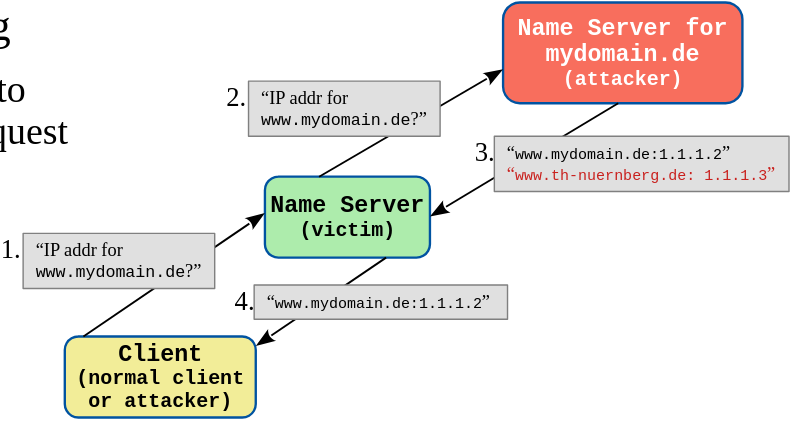
\includegraphics[width=0.7\columnwidth]{Resources/dns_poison1.png}

\paragraph{DNS Cache Poisoning: Fake Response Faster than Legitimate Server}
This attack involves the attacker sending a fake DNS response faster than the legitimate authoritative server. The steps are:
\begin{itemize}
    \item \textbf{Step 1:} The attacker sends a DNS query for a domain (e.g., \texttt{www.example.com}) to the victim's name server.
    \item \textbf{Step 2:} The victim forwards the query to the legitimate authoritative name server.
    \item \textbf{Step 3:} The attacker sends a forged response containing a malicious IP address before the legitimate server can reply.
    \item \textbf{Step 4:} The victim name server caches the fake response and returns it to the attacker.
\end{itemize}
The result is that the legitimate response is ignored, and the malicious IP address is cached. Countermeasures include randomizing ports and query IDs, implementing DNSSEC, and stricter validation rules.

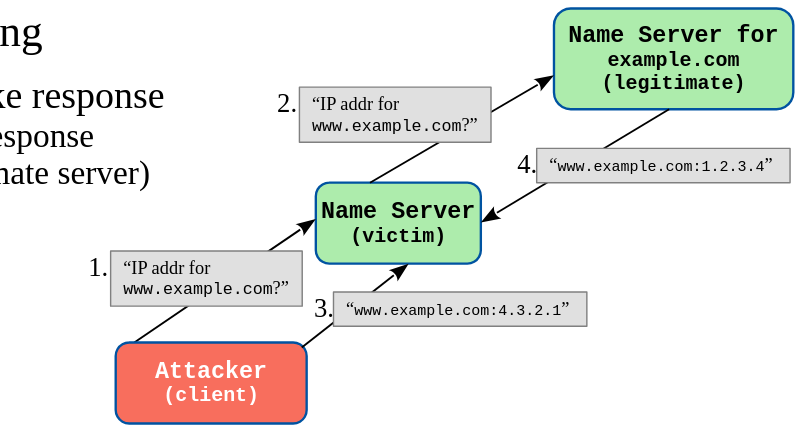
\includegraphics[width=0.7\columnwidth]{Resources/dns_poison2.png}

\paragraph{Kaminsky Attack}
The Kaminsky attack is a sophisticated DNS cache poisoning technique that exploits a vulnerability in DNS protocol design to inject malicious entries into DNS caches. The steps are as follows:
\begin{itemize}
    \item \textbf{Step 1:} The attacker repeatedly queries the victim name server for non-existent subdomains (e.g., \texttt{xyz123.example.com}).
    \item \textbf{Step 2:} The victim name server forwards the query to the authoritative server but receives a fake response from the attacker instead.
    \item \textbf{Step 3:} The fake response contains an authoritative NS record pointing to a malicious name server controlled by the attacker.
    \item \textbf{Step 4:} The victim caches the malicious name server as authoritative for the domain.
    \item \textbf{Step 5:} All subsequent DNS queries for the domain are redirected to the attacker's malicious name server.
\end{itemize}
This attack is particularly dangerous as it allows the attacker to poison entire DNS zones, redirecting all traffic for affected domains. Mitigations include randomizing query IDs, query source ports, and deploying DNSSEC to authenticate responses.

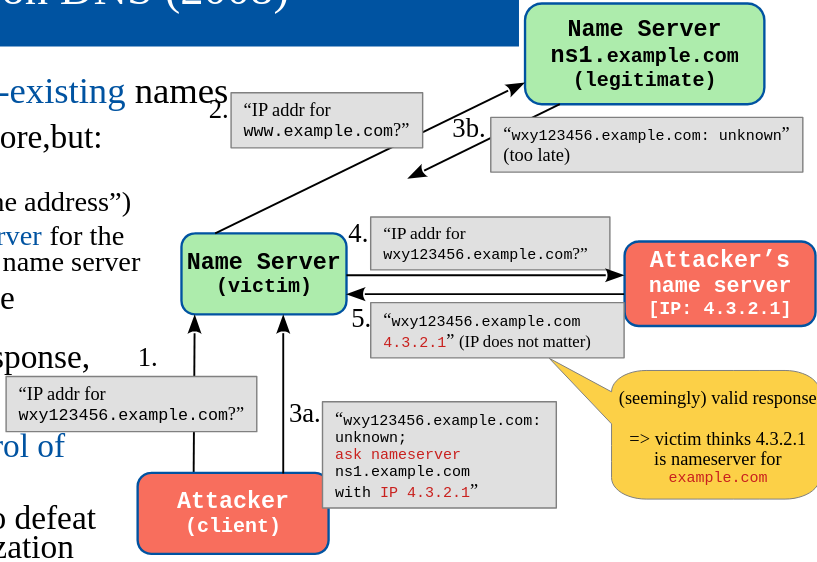
\includegraphics[width=0.6\columnwidth]{Resources/kaminsky.png}

\paragraph{Countermeasures Against DNS Cache Poisoning}
To protect against DNS cache poisoning and related attacks, the following countermeasures are commonly implemented:
\begin{itemize}
    \item \textbf{Randomized Query IDs:} Use randomized 16-bit query IDs to reduce predictability.
    \item \textbf{Randomized Source Ports:} Use random UDP source ports to add an additional layer of entropy.
    \item \textbf{DNSSEC:} Deploy DNSSEC to authenticate DNS responses and ensure their integrity.
    \item \textbf{Rate Limiting:} Implement rate limiting for queries and responses to reduce the likelihood of brute-force attacks.
    \item \textbf{Strict Validation:} Enforce strict validation rules for DNS responses.
\end{itemize}

These countermeasures significantly increase the difficulty for attackers to successfully perform DNS cache poisoning or similar attacks.

\subsubsection{DNSSEC (Domain Name System Security Extensions)}
\textbf{Goal of DNSSEC:}
\begin{itemize}
    \item \textbf{Origin Authentication:} Ensures authenticity of DNS data.
    \item \textbf{Authenticated Denial of Existence:} Proof of non-existence of records.
    \item \textbf{Data Integrity:} Verifies DNS data has not been tampered with.
\end{itemize}
\textbf{History:}
\begin{itemize}
    \item 1993: Discussions and development started.
    \item 1997, 1999: Initial proposals (RFCs 2065, 2535, now obsolete).
    \item 2005: Current approach (RFCs 4033-4035).
    \item 2010: All root servers supported DNSSEC.
    \item 2011: DNSSEC adopted for \texttt{.de} domains.
\end{itemize}
\textbf{Key Resource Records Introduced:}
\begin{itemize}
    \item \textbf{DNSKEY:} Public keys for signing zone data, distinguishing Key Signing Keys (KSK) and Zone Signing Keys (ZSK).
    \item \textbf{DS:} Delegation Signer; links parent to child zones.
    \item \textbf{RRSIG:} Digital signatures for verifying records.
    \item \textbf{NSEC/NSEC3:} Proof of non-existence through authenticated linked lists of DNS records.
\end{itemize}
\textbf{General Procedure:}\\
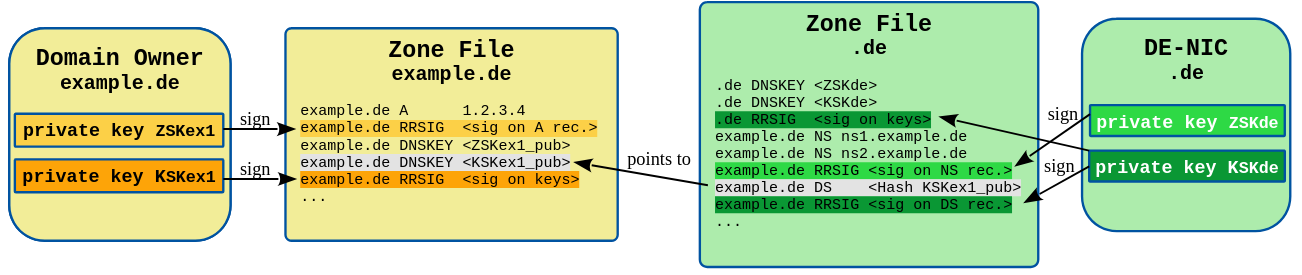
\includegraphics[width=\columnwidth]{Resources/dnssec.png}
\begin{enumerate}
    \item Zone entries are signed with private ZSK.
    \item ZSK is signed by private KSK.
    \item Parent domain stores the hash of the child zone’s KSK in a DS record.
    \item Establishes a recursive \textit{chain of trust}, starting from the root zone.
    \item Public key of the root zone acts as the \textit{trust anchor}.
\end{enumerate}
\textbf{Chain of Trust:}
\begin{itemize}
    \item Starts at the root zone.
    \item Extends through TLDs, domain zones, and subdomains.
    \item Requires the public key of the root zone to be securely distributed.
\end{itemize}
\paragraph{NSEC: Proof of Non-Existence}
\begin{itemize}
    \item Authenticates denial of existence by creating a sorted linked list of all domain names in a zone.
    \item Each signed entry includes the next domain name.
    \item Example: If \texttt{hello.example.com} is queried but doesn't exist, the response includes proof of its neighboring domains.
    \item \textbf{Disadvantage:} Enables zone walking, where attackers can list all (sub-)domains.
\end{itemize}
\paragraph{NSEC3: Mitigation of Zone Walking}
\begin{itemize}
    \item Uses hashed domain names instead of plaintext.
    \item Sorted hashes prevent attackers from easily enumerating domain names.
    \item Clients compute the hash of the requested domain and compare it to NSEC3 records.
    \item Dictionary attacks are still possible, but mitigated using salt and multiple hashing iterations.
\end{itemize}
\paragraph{Other Uses of DNSSEC}
DNSSEC can be utilized to enhance other security mechanisms by securely distributing associated data:
\begin{itemize}
    \item \textbf{SSH fingerprints:} Distributed as per RFC 4244.
    \item \textbf{IPsec/IKE public keys:} Defined in RFC 4025.
    \item \textbf{TLS trust anchors via DANE (RFC 6698):}
    \begin{itemize}
        \item DNS-Based Authentication of Named Entities (DANE).
        \item Protects against clandestine TLS certificate exchange by attackers.
        \item Enables referencing of X.509 certificates in DNSSEC-protected resource records (TLSA records).
    \end{itemize}
\end{itemize}
\paragraph{DNSSEC in Practice}
\begin{itemize}
    \item \textbf{Slow Adoption:} DNSSEC uptake has been slow due to:
    \begin{itemize}
        \item Overhead in communication, computation, delays, and administrative effort.
        \item Limited operational experience despite its long history.
        \item Larger resource records, increasing the potential for DoS attacks.
    \end{itemize}
    \item \textbf{No Confidentiality:} DNSSEC was not designed to provide confidentiality.
    \item \textbf{Typical Deployment:}
    \begin{itemize}
        \item The resolver is usually the nameserver of the ISP or network, not the local system.
        \item Resolver verifies signatures but requires the path from the end-user system to the resolver to be secured.
    \end{itemize}
\end{itemize}
\subsubsection{DNS-over-TLS (DoT) and DNS-over-HTTPS (DoH)}
\begin{itemize}
    \item \textbf{DNS-over-TLS (DoT):}
    \begin{itemize}
        \item Uses \textbf{TLS} (instead of UDP) to transport DNS queries.
        \item Provides \textbf{confidentiality}, integrity, and authenticity between the client and resolver (nameserver, often referred to as the ``DNS provider'').
        \item Does not protect traffic between nameservers (e.g., between the DNS provider and the authoritative nameserver).
    \end{itemize}
    \item \textbf{DNS-over-HTTPS (DoH):}
    \begin{itemize}
        \item Similar to DoT but uses \textbf{HTTPS} to send queries via POST or GET requests.
        \item Supports normal query formats (as used in UDP) or even JSON.
        \item Particularly suited for browsers and web applications.
        \item Comes with \textbf{additional overhead and dependencies}.
    \end{itemize}
\end{itemize}
\subsection{Zusammenfassung DNS}
\begin{itemize}
    \item \textbf{Domain Name System (DNS)}
    \begin{itemize}
        \item Developed without security in mind
        \item Vulnerabilities: \textbf{Cache poisoning attacks}, Kaminsky's attack
    \end{itemize}
    \item \textbf{DNSSEC}
    \begin{itemize}
        \item Provides \textbf{digital signatures and keys} in DNS resource records
        \item Ensures \textbf{integrity} and \textbf{authenticity} of DNS responses
        \item Implements \textbf{NSEC/NSEC3} for proof of non-existence of DNS names
        \item Can bootstrap other security mechanisms
    \end{itemize}
    \item \textbf{DNS-over-HTTPS (DoH)}, \textbf{DNS-over-TLS (DoT)}
    \begin{itemize}
        \item Protect traffic from the end user system to the DNS resolver / nameserver
        \item Both provide \textbf{confidentiality, integrity, and authenticity} via \textbf{TLS}
    \end{itemize}
\end{itemize}

\section{eMail and Messaging Security}
\subsection{eMail}
\subsubsection{Sending Emails: SMTP, POP3, IMAP}
\begin{itemize}
    \item \textbf{Protocols:}
    \begin{itemize}
        \item Send: SMTP (Simple Mail Transfer Protocol)
        \item Receive: POP3 or IMAP
    \end{itemize}
    \item \textbf{Security:}
    \begin{itemize}
        \item \textbf{TLS:} 
        \begin{itemize}
            \item SMTP over TLS: sender to mail server
            \item POP3/IMAP over TLS: mail server to recipient
        \end{itemize}
        \item \textbf{Between Mail Servers:} Opportunistic encryption (e.g., STARTTLS)
        \begin{itemize}
            \item Starts unprotected, upgrades to TLS if supported.
            \item Falls back to plaintext if TLS fails.
            \item No identity verification (certificates often not checked).
        \end{itemize}
    \end{itemize}
\end{itemize}

\subsubsection{PGP: End-to-End Security for Emails}
\begin{itemize}
    \item \textbf{Pretty Good Privacy (PGP):}
    \begin{itemize}
        \item Developed in 1991 by Phil Zimmermann.
        \item Signs and encrypts data (not limited to email).
        \item Standardized as OpenPGP (RFC 2440, 4880).
        \item Implementations: commercial PGP, GnuPG (open source), others.
        \item Trust model: Web of Trust (decentralized, ``anarchic'').
    \end{itemize}
    
    \item \textbf{End-to-End Security:}
    \begin{itemize}
        \item Hybrid encryption:
        \begin{itemize}
            \item Symmetric key (session-specific) encrypted by recipient's public key.
            \item Message encrypted with the symmetric key.
        \end{itemize}
        \item \textbf{Independent Signature \& Encryption:}
        \begin{itemize}
            \item PGP handles signing and encryption as separate operations.
            \item Issue: Without binding the signature to the encryption context, attackers can:
            \begin{itemize}
                \item Remove encryption and present the signature in plaintext (signature repudiation).
                \item Forward signed plaintext to unintended recipients without the encryption.
                \item Modify unsigned metadata or associate it with a different context.
            \end{itemize}
            \item Modern cryptographic standards prefer combining these operations into a single, secure AEAD process to ensure both confidentiality and integrity.
        \end{itemize}
        \item \textbf{Authenticated Encryption (AE):}
        \begin{itemize}
            \item Introduced in 2001 as a partial fix (Modification Detection Code, MDC).
            \item MDC ensured detection of tampering but lacked proper AE guarantees.
            \item Issues with early AE:
            \begin{itemize}
                \item MDC was not strongly integrated into the cryptographic protocol.
                \item Attacks possible if MDC was not always applied correctly.
            \end{itemize}
            \item Recent standards include ``real'' AEAD (Authenticated Encryption with Associated Data):
            \begin{itemize}
                \item Combines encryption and integrity into a single operation.
                \item Protects both the ciphertext and associated metadata (e.g., headers).
                \item Ensures signatures cannot be separated from encryption.
            \end{itemize}
        \end{itemize}
    \end{itemize}
    
    \item \textbf{Main Critiques:}
    \begin{itemize}
        \item Usability issues: easy to misuse.
        \item Poor integration with many mail clients.
    \end{itemize}
\end{itemize}

\subsubsection{MIME, PGP/MIME, S/MIME}
\begin{itemize}
    \item \textbf{MIME (Multi-purpose Internet Mail Extensions):}
    \begin{itemize}
        \item Enables email attachments and sending arbitrary data (not just text).
        \item MIME header specifies transfer encoding and content type (MIME type).
    \end{itemize}
    \item \textbf{PGP/MIME:}
    \begin{itemize}
        \item Allows sending PGP-encrypted or signed ciphertext as MIME attachments.
    \end{itemize}
    \item \textbf{S/MIME (Secure MIME):}
    \begin{itemize}
        \item Alternative solution for encrypting and signing emails.
        \item Based on X.509 certificates and Public Key Infrastructure (PKI).
        \item Provides encryption and signing with properties similar to PGP but utilizes a different trust model.
    \end{itemize}
\end{itemize}

\subsubsection{E-Mail End-to-End Security: S/MIME and PGP}
\begin{itemize}
    \item \textbf{Both S/MIME and PGP are widely used for secure email communication:}
    \begin{itemize}
        \item \textbf{S/MIME:} Better suited for corporate environments.
        \begin{itemize}
            \item Companies can distribute certificates to employees.
            \item IT departments can pre-configure email clients (e.g., install plugins).
            \item Users simply click to encrypt/sign emails.
            \item Works seamlessly within the organization's infrastructure.
        \end{itemize}
        \item \textbf{PGP:} Decentralized, popular among individuals and open-source communities.
        \begin{itemize}
            \item No need for a centralized PKI; individuals maintain control.
            \item Less user-friendly and more error-prone than S/MIME.
        \end{itemize}
    \end{itemize}
    \item \textbf{Efail attack (2018):} Affected both S/MIME and PGP by exploiting how email clients handled encrypted content.
\end{itemize}

\subsubsection{Improving Transport Encryption for Email}
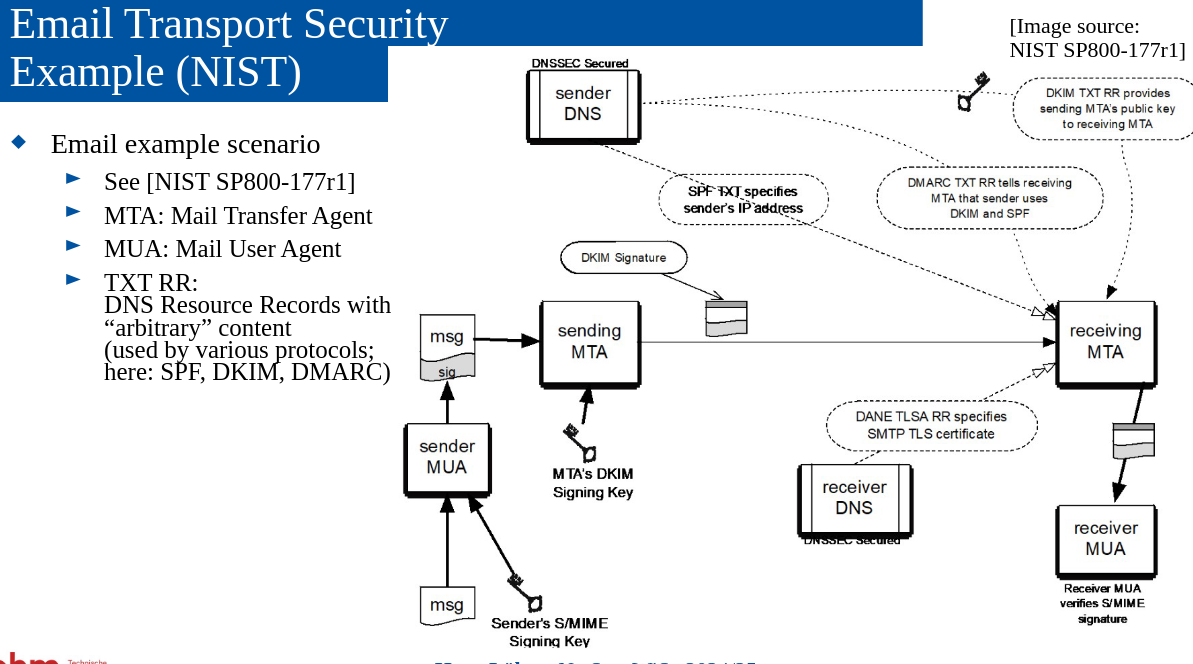
\includegraphics[width=\columnwidth]{Resources/mail.png}
\textbf{DANE (DNS-based Authentication of Named Entities)}  
\begin{itemize}
    \item DNS entry (TLSA record) acts as a trust anchor for TLS certificate verification.
    \item Requires DNSSEC to ensure integrity.
    \item Prevents downgrade attacks by enforcing TLS if TLSA records are available.
\end{itemize}
\textbf{SPF, DKIM, and DMARC}  
\begin{itemize}
    \item \textbf{SPF:} Specifies authorized mail servers for a domain.
    \item \textbf{DKIM:} Signs outgoing emails with private keys; recipients verify signatures.
    \item \textbf{DMARC:} Combines SPF and DKIM, defines policies for authentication and reporting.
\end{itemize}
\textbf{MTA-STS (MTA Strict Transport Security)}  
\begin{itemize}
    \item Alternative to DANE, uses a "trust on first use" (TOFU) approach.
    \item Does not require DNSSEC.
\end{itemize}

\subsection{Instant Messaging: Signal Protocol}  
\begin{itemize}
    \item State-of-the-art security protocol for messaging, used by apps like WhatsApp.
    \item \textbf{History:}
    \begin{itemize}
        \item Developed by Open Whisper Systems (Moxie Marlinspike, Trevor Perrin) for \textit{TextSecure} (now Signal).
        \item Originates from \textit{Off-the-Record} (OTR) protocol $\rightarrow$ TextSecure v1 (2013).
        \item TextSecure v2 (2014): Introduced \textit{Axolotl Ratchet}.
        \item TextSecure v3 (2014): New cryptographic primitives and formats.
        \item Signal (2016): Protocol updated and renamed.
        \item Formal security analysis in 2016; published in 2017.
    \end{itemize}
\end{itemize}

\subsubsection*{Key Components}
\begin{itemize}
    \item \textbf{KDF Chain:} A Key Derivation Function (KDF) is used in a forward-only hash chain to ensure:
    \begin{itemize}
        \item \textit{Resilience:} Output keys appear random even if adversary controls inputs.
        \item \textit{Forward Security:} Past keys remain secure if current keys are compromised.
        \item \textit{Break-in Recovery:} Future keys remain secure with sufficient entropy.
    \end{itemize}
    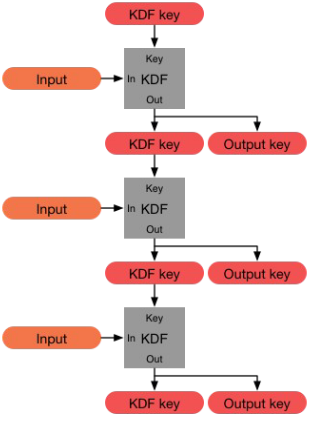
\includegraphics[width=0.4\columnwidth]{Resources/signal_kdf.png}
    
    \item \textbf{Double Ratchet Mechanism:} Combines two ratchets:
    \begin{itemize}
        \item \textit{Symmetric Key Ratchet:} Uses a KDF to generate encryption keys for messages.
        \item \textit{Diffie-Hellman (DH) Ratchet:} Updates DH key pairs for forward secrecy after every message exchange.
    \end{itemize}
    
    \item \textbf{Diffie-Hellman Ratchet:}
    \begin{itemize}
        \item Continuously performs DH key exchanges for each message.
        \item Transmits DH key shares with messages.
        \item Computes new shared secrets to derive message encryption keys.
    \end{itemize}
    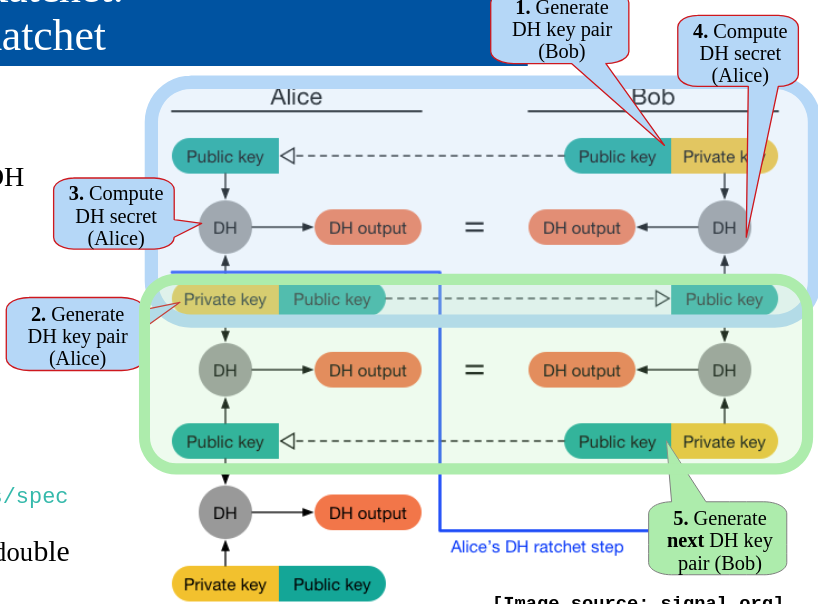
\includegraphics[width=0.8\columnwidth]{Resources/signal_dh.png}
    
    \item \textbf{Root Chain:} Combines the DH ratchet and symmetric key ratchet:
    \begin{itemize}
        \item Generates a root key (RK) through DH exchanges.
        \item Derives sending and receiving chain keys (CKs) for message encryption.
        \item Complete ratchet step => new root key
    \end{itemize}
    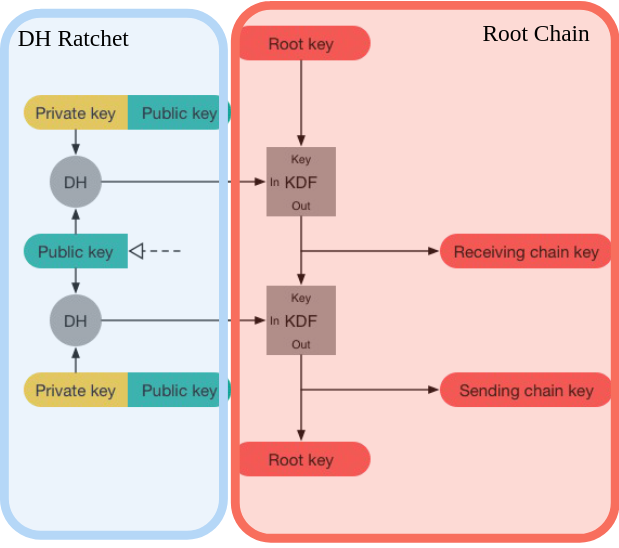
\includegraphics[width=.5\columnwidth]{Resources/signal_root_chain.png}
    
    \item \textbf{Message Keys:} Each message key is derived from the corresponding chain key (CK):
    \begin{itemize}
        \item Sender's CK encrypts messages.
        \item Receiver's CK decrypts messages.
        \item Ensures messages cannot be decrypted after keys are deleted.
    \end{itemize}
    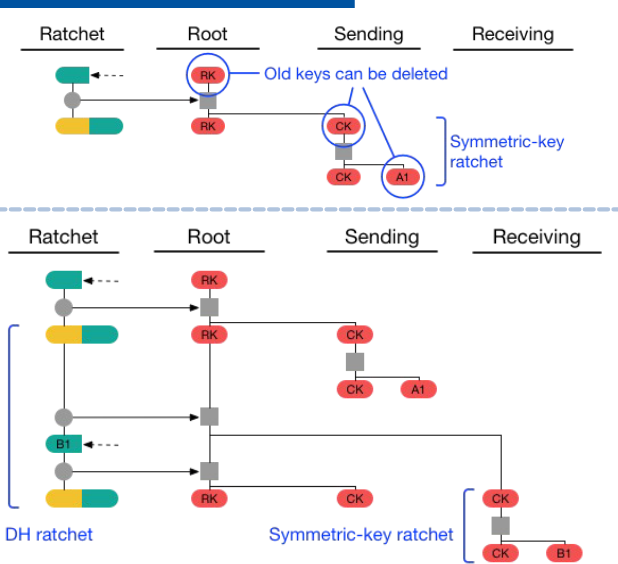
\includegraphics[width=0.8\columnwidth]{Resources/signal_message_keys.png}
\end{itemize}

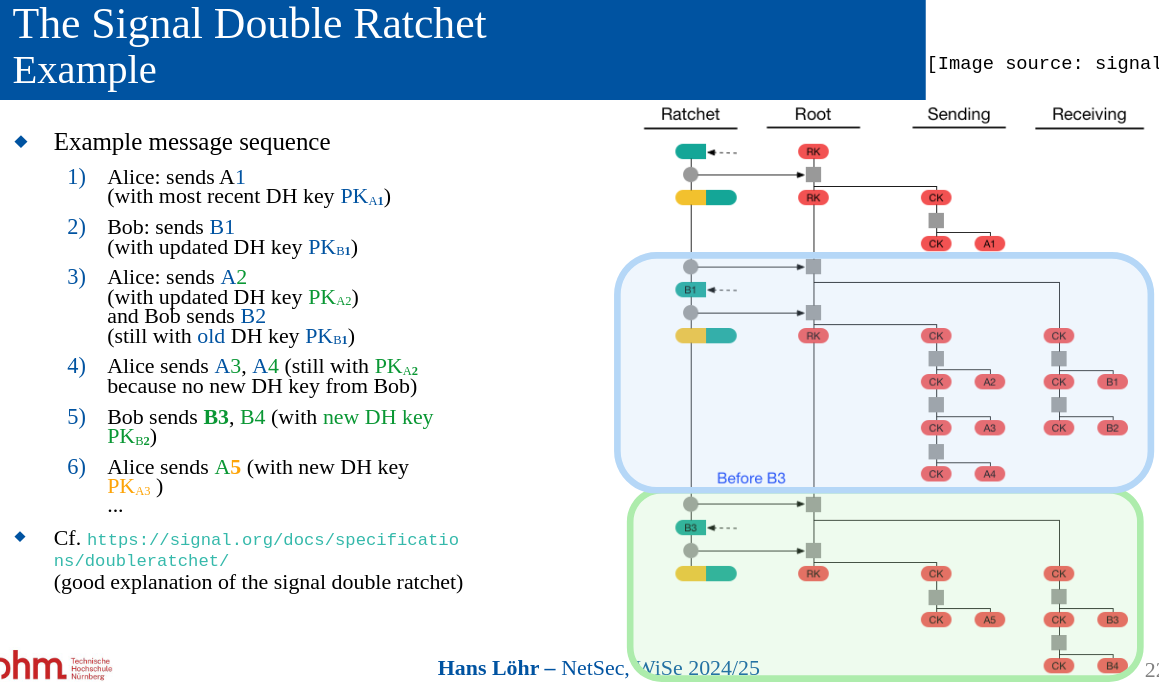
\includegraphics[width=.9\columnwidth]{Resources/signal_example.png}

\subsection{Summary: Email and Messaging Security}

\paragraph{Email Security}
\begin{itemize}
    \item \textbf{End-to-End Security:} 
    \begin{itemize}
        \item Practical but rarely used due to usability issues.
        \item Solutions: \textbf{PGP}, \textbf{S/MIME}.
    \end{itemize}
    \item \textbf{Email Transport Security:}
    \begin{itemize}
        \item Originally not designed with security in mind.
        \item Improvements: \textbf{DANE}, \textbf{SPF}, \textbf{DKIM}, \textbf{DMARC}.
    \end{itemize}
\end{itemize}

\paragraph{Instant Messaging Security}
\begin{itemize}
    \item \textbf{Modern Use Case:}
    \begin{itemize}
        \item Instant messaging is more recent compared to "ancient" email.
        \item Requires tailored security solutions.
    \end{itemize}
    \item \textbf{Closed Ecosystems:}
    \begin{itemize}
        \item Easier to deploy robust security.
        \item High dependency on service providers, limiting competition.
    \end{itemize}
    \item \textbf{Signal Protocol:}
    \begin{itemize}
        \item Designed for end-to-end security and confidentiality.
        \item Based on the \textbf{double ratchet} mechanism.
        \item Ensures forward secrecy; used by multiple messengers.
    \end{itemize}
\end{itemize}

\section{Anonymous Communication}

\subsection{Why Anonymous Communication?}
\begin{itemize}
    \item \textbf{Anonymity:} Unlinkability zwischen Nachricht/Aktion und Identität.
    \item \textbf{Arten:} Sender-Anonymität, Empfänger-Anonymität.
    \item \textbf{Anonymitätsset:} Gruppe möglicher, nicht unterscheidbarer Teilnehmer.
    \item \textbf{Vorteile:} Schutz der Privatsphäre, Meinungsfreiheit, Whistleblowing.
    \item \textbf{Nachteile:} Missbrauch (illegale Aktivitäten), Performance-Overhead.
\end{itemize}

\subsection{Dining Cryptographers (DC)}
\begin{itemize}
    \item \textbf{Szenario:} Drei Kryptographen möchten wissen, ob einer von ihnen bezahlt hat, ohne die Identität des Zahlenden zu offenbaren.
    \item \textbf{DC-Protokoll:} 
    \begin{itemize}
        \item Erlaubt das anonyme Senden eines Bits („jemand hat bezahlt“ / „niemand hat bezahlt“).
        \item Informations-theoretische Anonymität.
        \item Erweiterbar auf größere Gruppen (DC-Netzwerke).
        \item Hoher Aufwand, benötigt viel Zufälligkeit.
    \end{itemize}
    \item \textbf{Dissent:} Anonymes Kommunikationssystem basierend auf DC-Netzwerken, bietet nachweisbare Anonymitätsgarantien.
\end{itemize}
\noindent
\textbf{Prinzip:} Teilnehmer teilen Zufallsbits mit ihren Nachbarn.
\begin{itemize}
    \item \textbf{Bit-Berechnung:} XOR(links, rechts, eigene Nachricht).
    \item \textbf{Ergebnis:} Summe aller Bits (mod 2) zeigt an, ob eine Nachricht gesendet wurde.
    \item \textbf{Eigenschaften:}
    \begin{itemize}
        \item Informations-theoretische Anonymität.
        \item Erweiterbar auf mehrere Nachrichten (mehrere Runden).
        \item Hoher Overhead (jeder muss teilnehmen).
    \end{itemize}
\end{itemize}

\subsection{MixNets}
\begin{itemize}
    \item \textbf{Prinzip:} Nachrichten durchlaufen eine Kette von Mixen (\(M_0, M_1, M_2\)), wobei jede Schicht der Verschlüsselung entfernt wird.
      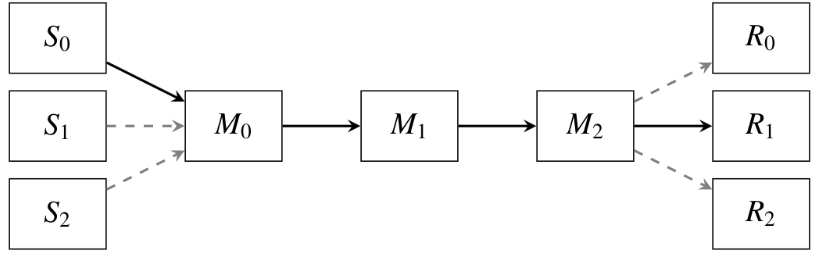
\includegraphics[width=.7\columnwidth]{Resources/mixes.png}
    \item \textbf{Ablauf:} 
    \[
    S_0 \to M_0: \text{enc}_{PK_{M_0}}(\text{enc}_{PK_{M_1}}(\text{enc}_{PK_{M_2}}(\text{enc}_{PK_{R_1}}(\text{msg}), R_1), M_2), M_1)
    \]
    \item \textbf{Eigenschaften:}
    \begin{itemize}
        \item Jedes Mix entschlüsselt nur eine Schicht und leitet die Nachricht weiter.
        \item Sender bestimmt die Reihenfolge der Mixe.
        \item Anonymität garantiert, solange mindestens ein Mix ehrlich ist.
    \end{itemize}
    \item \textbf{Herausforderungen:}
    \begin{itemize}
        \item Mix wartet auf alle Nachrichten → Geschwindigkeit hängt vom langsamsten Sender ab.
        \item Mix muss vertrauenswürdig sein (kennt Partner, aber nicht den Inhalt).
        \item Probleme:
        \begin{itemize}
            \item Zwei Sender adressieren denselben Empfänger.
            \item Ein Sender sendet mehrere Nachrichten.
            \item Ein Empfänger möchte antworten.
        \end{itemize}
    \end{itemize}
\end{itemize}

\subsection{Onion Routing und Tor}
\begin{itemize}
    \item \textbf{Problem von MixNets:} Zu langsam und ineffizient für Echtzeitkommunikation (z.B. TCP-Verbindungen).
    \item \textbf{Idee von Onion Routing:} 
    \begin{itemize}
        \item Aufbau eines \textbf{Circuits} von Sender zu Empfänger über Onion Routers (ORs).
        \item Sender wählt OR-Sequenz und baut symmetrische Sitzungsschlüssel mit Diffie-Hellman (DH) auf.
        \item Jeder OR kennt nur den vorherigen und nächsten OR (First OR kennt Sender, letzter OR den Empfänger).
        \item Datenübertragung erfolgt in „Schichten“ verschlüsselt (ähnlich MixNets).
    \end{itemize}
    \item \textbf{Tor:} Optimierte 2. Generation von Onion Routing.
    \begin{itemize}
        \item \textbf{TLS-geschützte Verbindungen} zwischen Relays (Schutz gegen passive Angriffe).
        \item Keine vollständige Sicherheit gegen Traffic-Analyse (z.B. Timing-Korrelationen).
        \item Directory Server (DS) zur Veröffentlichung der OR-Public Keys.
        \item Rate-Limiting und Staukontrolle verhindern Überlastung.
    \end{itemize}
    \item \textbf{Tor Hidden Services:}
    \begin{itemize}
        \item Server bleibt anonym, zensur- und DoS-resistent.
        \item Einführungspunkte (IP) und Rendezvous-Punkt (RP) vermitteln Kommunikation über Tor-Circuits.
    \end{itemize}
    \item \textbf{Nutzung von Tor:}
    \begin{itemize}
        \item Tor Browser, private Fenster (z.B. Brave), lokale Tor-Proxies oder Distributionen wie Tails.
        \item Achtung bei Betrieb von Tor-Relays, besonders Exit-Nodes (rechtliche Risiken).
    \end{itemize}
    \item \textbf{Einschränkungen:}
    \begin{itemize}
        \item Keine Sicherheit gegen Tracking auf Anwendungsebene (z.B. Browser-Fingerprinting).
    \end{itemize}
\end{itemize}

\section{WireGuard}

\subsection{Wichtige Merkmale}
\begin{itemize}
    \item \textbf{Kryptographie:}
    \begin{itemize}
        \item Moderne, sichere und geprüfte Kryptographie.
        \item Festgelegte Cipher-Suites: ChaCha20, Poly1305.
    \end{itemize}
    \item \textbf{Kleiner Codeumfang:}
    \begin{itemize}
        \item Nur ~4000 Zeilen Code im Linux-Kernel (OpenVPN ~120.000; IPsec ~400.000).
        \item Weniger Angriffsfläche und leichter auditierbar.
        \item Verzicht auf externe Kryptobibliotheken wie OpenSSL.
    \end{itemize}
    \item \textbf{Linux-Kernel-Integration:}
    \begin{itemize}
        \item Seit Kernel 5.6 (2020) fester Bestandteil des Linux-Kernels.
        \item Kein zusätzlicher Installationsaufwand oder Patches erforderlich.
        \item Minimaler Overhead, weniger Kontextwechsel als Userspace-VPNs.
    \end{itemize}
    \item \textbf{Performance:}
    \begin{itemize}
        \item Hohe Leistung bei vielen gleichzeitigen Verbindungen.
        \item Effizient auf Embedded Systems und einfachen Routern.
    \end{itemize}
    \item \textbf{Plattformunterstützung:}
    \begin{itemize}
        \item Implementierungen für Windows, macOS, Android, iOS, BSD-Systeme, Fritz!Box etc.
        \item Einfache Einrichtung durch \texttt{.conf}-Dateien und QR-Codes.
    \end{itemize}
\end{itemize}

\subsection{Modi und deren Einsatzarten}
\begin{itemize}
    \item \textbf{Tunnel-Modus:}
    \begin{itemize}
        \item Der gesamte IP-Verkehr wird durch den VPN-Tunnel geleitet.
        \item \textbf{Einsatzarten:}
        \begin{itemize}
            \item \textbf{Site-to-Site:} 
            \begin{itemize}
                \item Verbindung zwischen zwei Netzwerken.
                \item Beispiel: Firmenstandorte miteinander verbinden, um ein einheitliches Netzwerk zu schaffen.
            \end{itemize}
            \item \textbf{Site-to-End:}
            \begin{itemize}
                \item Verbindung zwischen einem Netzwerk und einem einzelnen Gerät.
                \item Beispiel: Remote-Arbeitsplätze mit Zugriff auf Unternehmensressourcen.
            \end{itemize}
        \end{itemize}
    \end{itemize}
    \item \textbf{Transport-Modus:}
    \begin{itemize}
        \item Nur bestimmte Protokolle oder Dienste werden durch den VPN-Tunnel geleitet.
        \item \textbf{Einsatzarten:}
        \begin{itemize}
            \item \textbf{End-to-End:}
            \begin{itemize}
                \item Direkte Verbindung zwischen zwei Geräten.
                \item Beispiel: Peer-to-Peer-Kommunikation, wie Dateiübertragungen oder sichere Anwendungen.
            \end{itemize}
        \end{itemize}
    \end{itemize}
\end{itemize}

\subsection{Protokollablauf}
\begin{itemize}
    \item \textbf{CryptoKey Routing:}
    \begin{itemize}
        \item Jede Netzwerkroute ist an einen öffentlichen Schlüssel gebunden.
        \item Nur autorisierte Datenpakete werden akzeptiert.
    \end{itemize}
    \item \textbf{Handshake:}
    \begin{itemize}
        \item Ephemerer Schlüsselaustausch (ECDH mit Curve25519).
        \item Sitzungsschlüssel durch HKDF abgeleitet; verwendet für ChaCha20 (Verschlüsselung) und Poly1305 (Authentifizierung).
        \item Optional: Pre-Shared Keys zur zusätzlichen Absicherung.
    \end{itemize}
    \item \textbf{Datenübertragung:}
    \begin{itemize}
        \item Pakete werden mit dem Sitzungsschlüssel verschlüsselt und enthalten einen WireGuard-Header (inkl. Typ, Key-ID, Counter, Payload, MAC).
    \end{itemize}
    \item \textbf{Key Rotation:}
    \begin{itemize}
        \item Schlüsselwechsel alle 120 Sekunden oder bei Erreichen von Limits (Counter/Data).
        \item Forward Secrecy durch Zeit- und Ressourcengesteuerte Schlüsselrotation.
    \end{itemize}
    \item \textbf{Reactivation:}
    \begin{itemize}
        \item Verbindung wird bei Inaktivität oder Unterbrechung neu aufgebaut (Handshake).
        \item Counter und alte Schlüssel werden aktualisiert.
    \end{itemize}
\end{itemize}

\subsection{Besonderheiten}
\begin{itemize}
    \item \textbf{Keep-Alive:}
    \begin{itemize}
        \item Hält Verbindungen aktiv, z. B. bei NAT oder mobilen Netzwerken.
        \item Konfigurierbar mit \texttt{PersistentKeepalive}.
    \end{itemize}
    \item \textbf{Sicherheit:}
    \begin{itemize}
        \item Schutz vor Replay-Angriffen durch Message Counter.
        \item Verschlüsselung aller Pakete, minimale Angriffsfläche durch kompakten Code.
    \end{itemize}
\end{itemize}

\section{Cyberangriffsmuster und -modelle}

\subsection{Attack Patterns}
\textbf{Definition:} Standardisierte Beschreibungen von Angriffstechniken, die zur Identifikation und Kategorisierung von Bedrohungen dienen.\\
\textbf{Historie:} Erste Cyberangriffe (Brain-Virus 1986, Morris-Wurm 1988) führten zur Notwendigkeit von Angriffsmuster-Klassifikationen. \\
\textbf{CAPEC:} \textit{Common Attack Pattern Enumeration and Classification}, entwickelt von MITRE seit 2007.

\subsection{Cyber Kill Chain (CKC)}
Ein Modell zur Beschreibung eines Cyberangriffs in sieben Phasen:
\begin{itemize}
    \item \textbf{Aufklärung (Reconnaissance):} Sammlung von Informationen über das Ziel (OSINT, Netzwerkscans).
    \item \textbf{Bewaffnung (Weaponization):} Erstellung schädlicher Nutzlasten (z.B. Exploits, Phishing-Dokumente).
    \item \textbf{Zustellung (Delivery):} Verbreitung der Schadsoftware (E-Mails, Drive-by-Downloads, USB-Sticks).
    \item \textbf{Ausnutzung (Exploitation):} Nutzung von Schwachstellen zur Code-Ausführung oder Privilegienerweiterung.
    \item \textbf{Installation (Installation):} Persistente Malware (Backdoors, Remote Access Trojaner).
    \item \textbf{Kommando und Kontrolle (C2):} Fernsteuerung kompromittierter Systeme über C2-Server.
    \item \textbf{Zielerreichung (Actions on Objectives):} Exfiltration, Erpressung oder Sabotage von Daten.
\end{itemize}

\subsection{MITRE ATT\&CK Framework}
\textbf{Beschreibung:} Seit 2015 öffentlich zugängliche Wissensbasis zur Dokumentation von Angriffstaktiken (Tactics) und Techniken (Techniques).\\
\textbf{Struktur:} 
\begin{itemize}
    \item Matrizen für verschiedene Plattformen (Enterprise, Mobile, ICS).
    \item \textbf{Tactic:} Ziel des Angriffs (z.B. Privilegienerweiterung).
    \item \textbf{Technique:} Methode zur Erreichung des Ziels (z.B. Pass-the-Hash).
\end{itemize}

\subsection{Anwendungen von MITRE ATT\&CK}
\begin{itemize}
    \item Verbesserung der Cyberabwehr durch Angriffsanalyse.
    \item Identifikation von Angreifergruppen anhand ihrer Techniken.
    \item Red- und Blue-Team-Übungen zur Angriffserkennung.
    \item Nutzung von Simulationstools wie \textit{Caldera}.
    \item Bessere Kommunikation mit Mitre codes (Publication, Virus total etc.)
\end{itemize}

\subsection{Weiterentwicklung von MITRE ATT\&CK}
\begin{itemize}
    \item Regelmäßige Updates durch Community-Beiträge.
    \item Verknüpfung mit CVEs zur besseren Bedrohungsbewertung.
    \item Erweiterung der Erkennungsmechanismen für ICS und Mobile Security.
    \item Fokus Social Engineering
\end{itemize}

\section{Zero Trust Networks}

\subsection{Definition}
\textbf{Zero Trust} ist ein Sicherheitsmodell, das auf dem „Assume Breach“-Prinzip basiert. Es minimiert Rechte für alle Entitäten in einer Infrastruktur und setzt auf kontinuierliche Überprüfung und Validierung.

\subsection{Kernprinzipien}
\begin{itemize}
    \item \textbf{Kontinuierliche Überwachung und Validierung} aller Nutzer, Geräte und Anwendungen.
    \item \textbf{Prinzip der minimalen Rechtevergabe}, um die Angriffsfläche zu minimieren.
    \item \textbf{Annahme eines Datenlecks} als Standardannahme.
\end{itemize}

\subsection{Perimeter- vs. Zero Trust Modell}
\textbf{Perimeter-Modell:} Vertrauen basiert auf Netzwerkgrenzen, Nutzer innerhalb des Netzwerks gelten als vertrauenswürdig.\\
\textbf{Zero Trust Modell:} Kein implizites Vertrauen, Authentifizierung und Autorisierung erfolgen kontinuierlich für jede Anfrage.

\subsection{Funktionsweise von Zero Trust}
\begin{itemize}
    \item \textbf{Authentifizierung:} Identitätsprüfung durch:
    \begin{itemize}
        \item Etwas, das man weiß (Passwort)
        \item Etwas, das man besitzt (Token, Smartcard)
        \item Etwas, das man ist (Biometrie)
        \item Verhaltenserkennung
    \end{itemize}
    \item \textbf{Single Sign-On (SSO):} Nutzung von Protokollen wie Kerberos, OAuth, OpenID Connect (OIDC).
    \item \textbf{Gerätevertrauen:} Überprüfung durch Secure Boot, TPM, Gerätezertifikate.
    \item \textbf{Sichere Kommunikation:} Nutzung von TLS (Client-Server) und IPSec (Server-Server).
    \item \textbf{Erstpaket-Filterung (Bootstrapping Trust):} Sicherheitsprüfung bereits bei der ersten Netzwerkkommunikation.
    \item \textbf{Dynamische Richtliniendurchsetzung:} Zugriffskontrolle basierend auf Echtzeit-Analysen und Risiko-Bewertungen.
\end{itemize}

\subsection{Praktische Implementierungen}
\begin{itemize}
    \item \textbf{BeyondCorp (Google):} Nutzer- und Gerätetrust unabhängig vom Standort.
    \item \textbf{Microsoft Zero Trust Architektur:} Integration in Azure AD, Intune und Defender.
    \item \textbf{Cloudflare Zero Trust:} Kombination aus SASE und Zero Trust für Unternehmensnetzwerke.
\end{itemize}

\subsection{Vorteile von Zero Trust}
\begin{itemize}
    \item Schutz vor Insider-Bedrohungen und kompromittierten Konten.
    \item Granulare Zugriffskontrolle und geringere Angriffsfläche.
    \item Verbesserte Sichtbarkeit und Auditierbarkeit des Netzwerkverkehrs.
\end{itemize}

\section{Network Vulnerability Scanning}

\subsection{Definition}
\textbf{Vulnerability Scanning} ist der Prozess der Identifikation von Schwachstellen in Netzwerken, Betriebssystemen und Anwendungen durch automatisierte Tools.

\subsection{Wichtige Schwachstellen-Scanner}
\begin{itemize}
    \item \textbf{Nmap} (Network Mapper): Open-Source-Netzwerkscanner (1997, Gordon Lyon). Funktionen:
    \begin{itemize}
        \item Port-Scanning
        \item Betriebssystem- und Dienstversionserkennung
        \item Netzwerk-Scanning
    \end{itemize}
    \item \textbf{Nessus}: Kommerzieller Schwachstellenscanner (1998, Tenable). Funktionen:
    \begin{itemize}
        \item Scans für OS, Netzwerkgeräte und Webanwendungen
        \item Compliance- und Konfigurationsanalysen
        \item Detaillierte Berichte mit Handlungsempfehlungen
    \end{itemize}
    \item \textbf{OpenVAS} (Open Vulnerability Assessment Scanner): Open-Source-Schwachstellenscanner (2006, Greenbone). Funktionen:
    \begin{itemize}
        \item Authentifizierte und nicht-authentifizierte Scans
        \item Schwachstellenmanagement und Berichterstellung
    \end{itemize}
    \item \textbf{Zmap}: Schneller Open-Source-Netzwerkscanner (2013). Funktionen:
    \begin{itemize}
        \item Internetweite Netzwerkscans in Rekordzeit
        \item Anpassbare Scan-Raten
    \end{itemize}
    \item \textbf{SAINT} (Security Administrator's Integrated Network Tool): Kommerzieller Netzwerkscanner (1998). Funktionen:
    \begin{itemize}
        \item Schwachstellenscans und Compliance-Analysen
        \item Zentralisierte Verwaltung
    \end{itemize}
    \item \textbf{SATAN} (Security Administrator Tool for Analyzing Networks): Netzwerksicherheits-Analysetool (1995). Funktionen:
    \begin{itemize}
        \item Automatisierte und Remote-Scans
        \item Anpassbare Scans und detaillierte Berichterstellung
    \end{itemize}
    \item \textbf{Metasploit}: Open-Source-Penetrationstest-Framework (2003, Harley David Moore). Funktionen:
    \begin{itemize}
        \item Sammlung von Exploits für Sicherheitsanalysen
        \item Payload-Generierung für verschiedene Angriffsvektoren
        \item Post-Exploitation-Funktionen
    \end{itemize}
\end{itemize}

\subsection{Das OSI-Schichtenmodell und Scanning}
\begin{itemize}
    \item Verschiedene Scanner arbeiten auf unterschiedlichen OSI-Schichten:
    \begin{itemize}
        \item \textbf{Netzwerkscans (Layer 3-4)}: Nmap, Zmap
        \item \textbf{Schwachstellenscans (Layer 4-7)}: OpenVAS, Nessus, Burp Suite
        \item \textbf{Exploit-Tests (Layer 7)}: Metasploit
    \end{itemize}
\end{itemize}

\subsection{Realität vs. Testumgebung}
\textbf{Testumgebung:}
\begin{itemize}
    \item Kontrollierte Bedingungen
    \item Vorhersehbare Ergebnisse
    \item Vereinfachte Analysen
\end{itemize}
\noindent
\textbf{Echte Netzwerke:}
\begin{itemize}
    \item Komplexe Netzwerklandschaften
    \item Unvorhersehbare Ergebnisse
    \item Unerwartete Probleme durch Sicherheitsmechanismen
\end{itemize}

\subsection{Herausforderungen und False Positives}
\begin{itemize}
    \item Nicht jede gemeldete Schwachstelle ist real.
    \item Beispiel: Eine Webanwendung wird als \textit{SQL-Injection-anfällig} erkannt, aber ein manueller Test mit \textit{SQLmap} bestätigt dies nicht.
    \item Lösung: Kombination von automatischen Scans mit manuellen Überprüfungen.
\end{itemize}

\section{Wireless IoT Communication Security}

\subsection{Zigbee – Grundlagen}
\textbf{Zigbee} ist ein drahtloses Protokoll auf Basis des \textbf{IEEE 802.15.4-Standards} für energieeffiziente, kurze Kommunikationsstrecken, häufig in IoT-Geräten.\\
\textbf{Hauptmerkmale:}
\begin{itemize}
    \item Niedriger Energieverbrauch
    \item Netzwerktopologien: \textbf{Stern, Baum, Mesh}
    \item Geeignet für Sensoren, Smart Home, Industrieautomation
\end{itemize}

\subsection{Zigbee-Netzwerkarchitektur}
\begin{itemize}
    \item \textbf{Koordinator:} Erstellt und verwaltet das Netzwerk, verteilt Schlüssel.
    \item \textbf{Router:} Leitet Daten weiter, keine Schlüsselverwaltung.
    \item \textbf{Endgerät:} Sensoren, Aktoren, oft energieeffizient (Schlafmodus).
\end{itemize}

\subsection{Sicherheitsmodelle in Zigbee}
\begin{itemize}
    \item \textbf{Verteiltes Sicherheitsmodell:} Jeder Knoten verwaltet eigene Schlüssel.
    \item \textbf{Zentralisiertes Sicherheitsmodell:} Vertrauenscenter verwaltet Schlüssel.
    \item \textbf{Sicherheitsmechanismen:}
    \begin{itemize}
        \item AES-128-Bit-Verschlüsselung
        \item Integritätsprüfung durch Message Integrity Codes (MIC)
        \item Authentifizierungsmechanismen
    \end{itemize}
\end{itemize}

\subsection{Haupt-Sicherheitsrisiken bei Zigbee}
\begin{itemize}
    \item \textbf{Schwache Authentifizierung:} Standardmäßig voreingestellte, schwache Schlüssel.
    \item \textbf{Fehlende Zugangskontrolle:} Unzureichender Schutz der Schlüssel.
    \item \textbf{Geräteübernahme:} Durch physischen oder Remote-Zugriff.
\end{itemize}

\subsection{Allgemeine Angriffsarten auf IoT-Netzwerke}
\begin{itemize}
    \item \textbf{Replay-Angriff:} Aufgezeichnete Daten erneut senden.
    \item \textbf{Spoofing:} Identität fälschen.
    \item \textbf{Jamming:} Kommunikation stören.
    \item \textbf{Man-in-the-Middle (MITM):} Abfangen und Manipulieren von Daten.
\end{itemize}

\subsection{Beispiele für Sicherheitsvorfälle}
\begin{itemize}
    \item \textbf{Mirai-Botnet:} DDoS-Angriffe über unsichere IoT-Geräte.
    \item \textbf{Angriffe auf Zigbee-Geräte:} Netzwerkschlüssel während des Pairings gestohlen.
    \item \textbf{SILEX-Malware:} Löscht Konfigurationsdaten von IoT-Geräten.
\end{itemize}

\subsection{Lösungsansätze und Best Practices}
\begin{itemize}
    \item \textbf{Starke Verschlüsselung und Schlüsselverwaltung:}
    \begin{itemize}
        \item AES-256-Verschlüsselung
        \item Hardware-Sicherheitsmodule (HSM)
        \item Diffie-Hellman für sicheren Schlüsselaustausch
    \end{itemize}
    \item \textbf{Authentifizierungs- und Zugangskontrollen:}
    \begin{itemize}
        \item Multi-Faktor-Authentifizierung (MFA)
        \item Rollenbasierte Zugangskontrolle (RBAC)
    \end{itemize}
    \item \textbf{Netzwerksegmentierung und Firewalls:}
    \begin{itemize}
        \item VLANs zur Trennung von IoT- und Unternehmensnetzwerken
        \item Dedizierte IoT-Firewalls
    \end{itemize}
    \item \textbf{Regelmäßige Updates und Patches:}
    \begin{itemize}
        \item Automatische Updates
        \item Rollback-Mechanismen zur Wiederherstellung nach fehlgeschlagenen Updates
    \end{itemize}
    \item \textbf{Zukunftstrends in der IoT-Sicherheit:}
    \begin{itemize}
        \item Hardwarebasierte Sicherheitslösungen (TPM, Secure Elements)
        \item Blockchain zur sicheren Geräteidentität
        \item Künstliche Intelligenz (KI) für Angriffserkennung
    \end{itemize}
\end{itemize}

